%\chapter{Synthetic Seismograms}
\chapter{理论地震图}
\label{chapter:SNREIgrams}

既然我们已经了解如何计算球对称无自转地球模型的本征频率及其相应的本征函数,
用简正模式叠加的方法来合成长周期地震图和频谱就成为一件简单的事情。
弹性或非弹性球对称地球的响应是所有非平凡球型和环型单态模式本征函数${}_n\bs_{lm}^{\rm S}$和${}_n\bs_{lm}^{\rm T}$的叠加。
在本章中,我们发展一个算子体系以便在普通的地理坐标系(而非震中坐标系)中能够对球谐函数级数~$m$直接求和。
我们将交替使用撇号(如$\bx'$)和下标s(如$\bx_{\rm s}$)两种符号来表示震源位置,
并在一开始的几何分析中使用前者。
在最终格林函数张量$\bG(\bx,\bx';t)$和
对位于$\bx_{\rm s}$的矩张量源$\bM$的位移响应$\bs(\bx,t)$的公式中,
对地球的非弹性做了完全的处理,因为这样做并不会使得推导过于复杂。

%\section{Source-Receiver Geometry}
\section{源点-接收点几何关系}
\index{source-receiver geometry|(}%
\label{section:10.1}

令$\brh$、$\bthetah$和$\bphih$为位于接收点$\bx$处的一组相互垂直的三个单位矢量,
其方向分别为半径$r$、余纬度$\theta$和经度$\phi$增加的方向,
而$\brh'$、$\bthetahpr$和$\bphihpr$则是在地震点源$\bx'$处对应的三个矢量,
其方向分别为$r'$、$\theta'$和$\phi'$增加的方向。
球对称地球响应的最简便的表达式是使用接收点和源点的半径$r$和$r'$,
以及一对震中坐标系中的角度坐标,我们用$\Theta$和$\Phi$来表示。
其中$\Theta$为源点和接收点之间的{\em 角震中距\/},
\index{angular epicentral distance}%
\index{epicentral distance}%
由下式给定
\eq
\cos\Theta=\brh\cdot\brh'=\cos\theta\cos\theta'
+\sin\theta\sin\theta'\cos(\phi-\phi'),
\label{eq:10.cosdelta}
\en
而$\Phi$则是接收点的{\em 方位角\/},
\index{azimuth}%
\index{source azimuth}%
在源点{\em 从正南方向\/}沿{\em 逆时针\/}方向测量。
对于一个固定的源点位置$\bx'$,我们可以把$r$、$\Theta$、$\Phi$
视为表述接收点位置的震中球极坐标系。
在大多数定量地震学讨论中,震中距用$\Delta$而非$\Theta$表示;
在本书中,我们用$\Delta$来表示多周面波
\index{orbit}%
\index{surface-wave orbit}%
或体波所走过的角距离(见第11.3-11.5节和12.5节)。

为方便起见,我们定义两个与经过接收点和源点在单位球面上的投影的大圆相切的单位矢量:
\eq
\bThetah=\bdel_{\!1}\Theta,\qquad
\bThetahpr=-\bdel_{\!\rm 1}^{\raise.1ex\hbox{$\scriptstyle\prime$}}\Theta,
\label{eq:10.definition}
\en
其中$\bdel_{\!1}=\bthetah\p_{\theta}+\bphih(\sin\theta)^{-1}
\p_{\phi}$ 和 $\bdel_{\!1}^{\raise.1ex\hbox{$\scriptstyle\prime$}}=\bthetahpr\p_{\theta'}+\bphihpr(\sin\theta')^{-1}\p_{\phi'}$ 分别为关于接收点和源点坐标的表面梯度。
\index{gradient!at source}%
\index{gradient!at receiver}%
用~(\ref{eq:10.cosdelta})式推导~(\ref{eq:10.definition}),
我们得到显式表达式
\eqa
\lefteqn{\bThetah=(\sin\Theta)^{-1}\{\bthetah
\,[\sin\theta\cos\theta'
-\cos\theta\sin\theta'\cos(\phi-\phi')]}
\nonumber \\
&&\mbox{}\qquad\qquad\qquad+\bphih\,\sin\theta'\sin(\phi-\phi')\},
\label{eq:10.bdh}
\ena
\eqa
\lefteqn{\bThetahpr=
(\sin\Theta)^{-1}\{\bthetahpr\,[-\cos\theta\sin\theta'
+\sin\theta\cos\theta'\cos(\phi-\phi')]}
\nonumber \\
&&\mbox{}\qquad\qquad\qquad+\bphihpr\sin\theta\sin(\phi-\phi')\}.
\label{eq:10.bdhs}
\ena
接收点处的单位矢量 $\brh$ 和 $\bThetah$ 与源点处的相应矢量 $\brh'$ 和 $\bThetahpr$
直接可以通过一个绕源点-接收点大圆极点的旋转联系起来:
\eq \label{eq:10.1}
\brh=\brh'\cos\Theta+\bThetahpr\sin\Theta,\qquad
\bThetah=-\brh'\sin\Theta+\bThetahpr\cos\Theta.
\en
要在接收点和源点分别得到震中坐标系中完备的相互垂直的三个单位矢量,
我们做如下定义
\eq
\label{eq:10.defn2}
\bPhih=\brh\times\bThetah,\qquad
\bPhihpr=\brh'\times\bThetahpr.
\en
(\ref{eq:10.1})式确保 $\bPhih=\bPhihpr$; 从物理上讲,这第三个矢量是源点-接收点大圆面的单位法向。
源点矢量 $\bThetahpr$和 $\bPhihpr$与方位角 $\Phi$有简单的关系
\eq \label{eq:10.Phi}
\bThetahpr=\bthetahpr\cos\Phi+\bphihpr\sin\Phi,
\qquad\bPhihpr=-\bthetahpr\sin\Phi
+\bphihpr\cos\Phi.
\en
同样地,我们可以用在接收点处测得的源点的反方位角来定义 $\bThetah$和 $\bPhih$, 但这在后续的推导中是不需要的。
图~\ref{10.fig.geom}简要地显示了我们所使用的坐标系约定。

\begin{figure}[t]
\centering
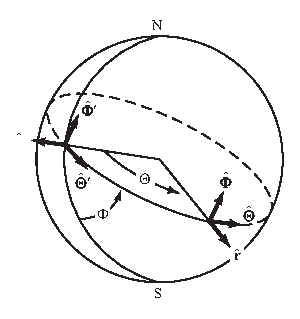
\includegraphics{../figures/chap10/fig01.eps}
\caption[SRgeometry]{
这里使用的坐标系约定示意图。
接收点位于 $\bx=(r,\theta,\phi)$,震源位于 $\bx'=(r',\theta',\phi')$。
为简单起见,图中显示的两个半径$r$和$r'$是相等的。
要注意的是,$\bThetah$ 和 $\bThetahpr$ 均指向从源点到接收点小弧的波传播方向。}
\label{10.fig.geom}
\end{figure}

$\brh$、$\bThetah$和$\bPhih$这三个方向分別对应于在
$x$点的地震仪的{\em 径向\/}、{\em 纵向\/}和{\em 横向\/}分量。
\index{component!radial}%
\index{component!longitudinal}%
\index{component!transverse}%
\index{radial component}%
\index{longitudinal component}%
\index{transverse component}%
\index{seismometer!radial component}%
\index{seismometer!longitudinal component}%
\index{seismometer!transverse component}%
这些关于接收点偏振的名称对地球自由振荡的研究是很自然的,
因为它们保留了球极坐标中"径向"一词常用的几何意义。
而在地震学日常用语中,习惯上称 $\bThetah$ 为"径向"方向,
$\brh$ 为"垂直"方向。
我们不会使用这些非正式名称,以免造成任何可能的混淆。

利用~(\ref{eq:10.bdh})--(\ref{eq:10.defn2})中的定义以及~(\ref{A.del1rhat})--(\ref{A.del1phat})中的几何等式,很容易证明:
\eq \label{eq:10.funny0}
\bdel_{\!1}\brh=\bThetah\bThetah+
\bPhih\bPhih,
\en
\eq
\bdel_{\!1}\bThetah=-\bThetah\brh+\bPhih\bPhih\cot\Theta,
\en
\eq
\bdel_{\!1}\bPhih=-\bPhih\brh-\bPhih\bThetah\cot\Theta,
\en
\eq
\bdel_{\!\rm 1}^{\raise.1ex\hbox{$\scriptstyle\prime$}}\brh'
=\bThetahpr\bThetahpr+
\bPhihpr\bPhihpr,
\en
\eq
\bdel_{\!\rm 1}^{\raise.1ex\hbox{$\scriptstyle\prime$}}
\bThetahpr=-\bThetahpr\brh'
-\bPhihpr\bPhihpr\cot\Theta,
\en
\eq
\bdel_{\!\rm 1}^{\raise.1ex\hbox{$\scriptstyle\prime$}}\bPhihpr=
-\bPhihpr\brh'
+\bPhihpr\bThetahpr\cot\Theta,
\en
\eq
\bdel_{\!1}\brh'=\bzero,
\en
\eq \label{eq:10.funny1}
\bdel_{\!1}\bThetahpr=
\bPhih\bPhihpr(\sin\Theta)^{-1},
\en
\eq \label{eq:10.funny2}
\bdel_{\!1}\bPhihpr=-\bPhih\bThetahpr(\sin\Theta)^{-1},
\en
\eq
\bdel_{\!\rm 1}^{\raise.1ex\hbox{$\scriptstyle\prime$}}\brh=\bzero,
\en
\eq \label{eq:10.funny3}
\bdel_{\!\rm 1}^{\raise.1ex\hbox{$\scriptstyle\prime$}}
\bThetah=-\bPhihpr\bPhih(\sin\Theta)^{-1},
\en
\eq \label{eq:10.funny4}
\bdel_{\!\rm 1}^{\raise.1ex\hbox{$\scriptstyle\prime$}}
\bPhih=\bPhihpr\bThetah(\sin\Theta)^{-1}.
\en
(\ref{eq:10.funny1})--(\ref{eq:10.funny2})两式表示的是因接收点坐标 $\theta$、 $\phi$的变化所引起的源点处切向矢量$\bThetahpr$、$\bPhihpr$的微扰,
而~(\ref{eq:10.funny3})--(\ref{eq:10.funny4})两式则表示因源点坐标$\theta'$、$\phi'$的变化所造成的接收点处矢量$\bThetah$、$\bPhih$的类似效应。

我们可以用震中距$\Theta$和方位角$\Phi$将接收点处的表面梯度算子$\bdel_{\!1}$表示成:
\eq
\bdel_{\!1}=(\bdel_{\!1}\Theta)\p_{\Theta}+(\bdel_{\!1}\Phi)\p_{\Phi}.
\label{eq:10.bdel}
\en
利用~(\ref{eq:10.Phi}) 和~(\ref{eq:10.funny1})两式,
我们得到
\eq
\bdel_{\!1}\Phi=(\sin\Theta)^{-1}\bPhih.
\label{eq:10.bdel1Phi}
\en
将~(\ref{eq:10.definition}) 和~(\ref{eq:10.bdel1Phi})
代入~(\ref{eq:10.bdel}) ,我们有
\eq
\bdel_{\!1}=\bThetah\hspace{0.2mm}\p_{\Theta}
+(\sin\Theta)^{-1}\bPhih\hspace{0.2mm}\p_{\Phi}.
\label{eq:10.bdel1}
\en
有鉴于 $r$、$\Theta$、$\Phi$ 构成一个震中球极坐标系,公式~(\ref{eq:10.bdel1}) 也可以根据第一性原理写出来。
\index{source-receiver geometry|)}%

%\section{Green Tensor}
\section{格林函数张量}
\index{tensor!Green!spherical Earth|(}%
\index{Green tensor!spherical Earth|(}%
\label{10.sec.Green}

在第6.2.3节中,我们已经将无自转非弹性地球模型的时间域格林函数张量用复数本征频率 $\nu_k=\om_k+i\gamma_k$ 及其本征函数 $\bs_k$ 来表示
\eq
\bG(\bx,\bx';t)=\real\sum_k(i\nu_k)^{-1}
\bs_k(\bx)\bs_k(\bx')\exp(i\nu_kt).
\label{eq:10.green1}
\en
对于球对称地球,角标$k$表示四元组合$\{n,l,m,\mbox{S 或 T}\}$,
其中$n$为径向阶数,$l$为球谐函数次数,$m$是球谐函数级数。
球型和环型本征频率${}_n\nu_l^{\rm S}={}_n\om_{lm}^{\rm S}+i{}_n\gamma_{lm}^{\rm S}$
和${}_n\nu_l^{\rm T}={}_n\om_{lm}^{\rm T}+i{}_n\gamma_{lm}^{\rm T}$与级数$m$ 无关,因此是$2l+1$重简并的。
对应的单态模式本征函数 ${}_n\bs_{lm}^{\rm S}$ 和
${}_n\bs_{lm}^{\rm T}$ 可以用~(\ref{8.realYdef})中的实数表面球谐函数表示为
\eq
\bs_k(\bx)=\bsDnl(r,\theta,\phi)\ylm(\theta,\phi),
\label{eq:10.bsk}
\en
其中,对于每一固定的阶数 $n$ 和球谐函数级数 $l$,
\eq
\bsD=\sU\brh+\sqLinv\sV\bdel_{\!1}
-\sqLinv\sW(\brh\times\bdel_{\!1}).
\label{eq:10.bsD}
\en
严格的位移算子$\bsD$是不依赖于$m$的,
\index{displacement operator}%
\index{operator!displacement}%
而且也是复数的,因为正如第9.9节所讨论的,球对称非弹性地球的径向本征函数$\sU$、$\sV$和$\sW$是复数的。为简洁起见,我们在下文中使用同一符号$\bsD$,
而不再分别定义球型和环型算子$\bsD^{\rm S}$ 和 $\bsD^{\rm T}$。
根据定义,在(\ref{eq:10.bsD})中环型模式的$\sU$和$\sV$为零,
球型模式的$\sW$为零。在源点处,与~(\ref{eq:10.bsk})--(\ref{eq:10.bsD})类似的公式为
\eq \label{eq:10.bskpr}
\bs_k(\bx')=\bsDnl'(r',\theta',\phi')\ylm(\theta',\phi')
\en
其中
\eq
\bsD'=\sU'\brh'+\sqLinv\sV'
\bdel_{\!1}^{\raise.1ex\hbox{$\scriptstyle\prime$}}
-\sqLinv\sW'(\brh'\times\bdel_{\!1}^{\raise.1ex\hbox{$\scriptstyle\prime$}}).
\en
径向本征函数$\sU'$,$\sV'$和$\sW'$上的撇号标示它们是在半径$r'$处取值。

将~(\ref{eq:10.bsk}) 和~(\ref{eq:10.bskpr})两个表达式 代入~(\ref{eq:10.green1}),我们可以将球对称非弹性地球上的格林函数张量写为
\eq
\bG(\bx,\bx';t)=\real\sum_{n=0}^\infty\sum_{l=0}^\infty
(i\nunl)^{-1}{}_n\bsG_l(\bx,\bx')\exp(i\nunl t).
\label{eq:10.finGreen}
\en
(\ref{eq:10.finGreen})式中与时间无关的张量 ${}_n\bsG_l(\bx,\bx')$为
\eq \label{10.Greeny}
\bsG=\bsD\,\bsD'
\sum_{m=-l}^{l}\ylm(\theta,\phi)
\ylm(\theta',\phi').
\en
(\ref{10.Greeny})式中对$m$的求和
可以用表面球谐函数的加法定理~(\ref{B.realaddth})来计算,其结果为
\eq \label{10.Greeny2}
\bsG=\left(\frac{2l+1}{4\pi}\right)
\bsD\,\bsD'\,P_l(\cos\Theta).
\en
从~(\ref{10.Greeny2}) 的形式显然有
\eq \label{10.recip}
\bsG(\bx,\bx')=\bsG^{\rm T}(\bx',\bx),
\en
因此表达式~(\ref{eq:10.finGreen}) 满足源点-接收点互易关系$\bG(\bx,\bx';t)=\bG^{\rm T}(\bx',\bx;t)$,t),这是必然的。
(\ref{eq:10.finGreen})中的求和包含所有非平凡球型和环型多态模式${}_n{\rm S}_l$和${}_n{\rm T}_l$。

要得到张量$\bsG$的一个适合数值计算的形式,
我们必须确定算子$\bsD$和$\bsD'$对勒让德多项式$P_l(\cos\Theta)$的作用。
利用~(\ref{eq:10.funny0})--(\ref{eq:10.funny4})中的结果和下面的等式
\eq \label{10.Pneed}
\bdel_{\!1}P_{l0}=-P_{l1}\bThetah,\qquad
\bdel_{\!1}P_{l1}=\half(\sqL^2P_{l0}-P_{l2})\bThetah,
\en
\eq \label{10.Pneed2}
\bdel_{\!\rm 1}^{\raise.1ex\hbox{$\scriptstyle\prime$}}P_{l0}
=P_{l1}\bThetahpr,\qquad
\bdel_{\!\rm 1}^{\raise.1ex\hbox{$\scriptstyle\prime$}}P_{l1}
=-\half(\sqL^2P_{l0}-P_{l2})\bThetahpr,
\en
其中$P_{lm}(\cos\Theta)$是级数为~$m$的连带勒让德函数,很容易证明
\eqa \label{10.ugly}
\lefteqn{\bsG=\left(\frac{2l+1}{4\pi}\right)
\biggl[\sU\hspace{0.2 mm}\sU'\brh\brh'P_{l0}
+\sqLinv(\sU\hspace{0.2 mm}\sV'\brh\bThetahpr
-\sV\hspace{0.2 mm}\sU'\bThetah\brh')P_{l1}} \nonumber \\
&&\mbox{}+\half\sqL^{-2}(\sV\hspace{0.2 mm}\sV'
\bThetah\bThetahpr+\sW\hspace{0.2 mm}\sW'\bPhih
\bPhihpr)(\sqL^2P_{l0}-P_{l2}) \nonumber \\
&&\mbox{}\qquad+\sqL^{-2}(\sV\hspace{0.2 mm}\sV'\bPhih\bPhihpr
+\sW\hspace{0.2 mm}\sW'\bThetah\bThetahpr)
(\sin\Theta)^{-1}P_{l1}\biggr].
\ena
所有涉及球型和环型本征函数乘积的项都消失了,
因为只要$\sW'$不为零,$\sU$和$\sV$就都为零,反之亦然。
在验证~(\ref{10.ugly})式满足对称性~(\ref{10.recip})时,
必须记住,当$\bx$和$\bx'$互换时,切向矢量$\bThetah$、$\bPhih$和 $\bThetahpr$、$\bPhihpr$会改变符号。

作为结束,我们提醒读者注意在~(\ref{eq:10.bsk})和~(\ref{eq:10.bskpr})这两个表达式中 使用实数表面球谐函数$\sY_{lm}$的必要性。
\index{spherical harmonics!real}%
\index{real spherical harmonics}%
如果我们轻率地采用了复数球谐函数$Y_{lm}$,我们将会在~(\ref{10.Greeny})中得到一个非旋转不变的求和$\sum_mY_{lm}(\theta,\phi)Y_{lm}(\theta',\phi')$。
非弹性本征函数$\bs_k$中唯一的复数性一定来自于$\sU$、$\sV$和$\sW$这些径向标量;
这是由~(\ref{6.orthog})--(\ref{6.normal})这两个双正交归一关系所决定的,如第9.9节中所述。
关于有无非弹性时模式叠加格林函数张量$\bG$基本性质的进一步说明,请参见第6.3.3节。
\index{tensor!Green!spherical Earth|)}%
\index{Green tensor!spherical Earth|)}%

%\section{Moment-Tensor Response}
\section{矩张量响应}
\index{moment-tensor response!spherical Earth|(}%
\index{response!spherical Earth|(}%

无自转非弹性地球对位于$\bx_{\rm s}$ 处的阶跃函数矩张量源$\bM$的位移响应为
\eq
\bs(\bx,t)=\real\sum_k\nu_k^{-2}\bM\!:\!\beps_k(\bx_{\rm s})
\,\bs_k(\bx)\,[1-\exp(i\nu_kt)],
\label{eq:10.acc1}
\en
其中 $\beps_k=\half[\bdel\bs_k+(\bdel\bs_k)^{\rm T}]$ 为应变.
将~(\ref{eq:10.bsk})和~(\ref{eq:10.bskpr})中球对称地球本征函数$\bs_k(\bx)$和$\bs_k(\bx_{\rm s})$ 的表达式代入,
并像第10.2节中一样应用球谐函数加法定理,我们可以将~(\ref{eq:10.acc1})写为
\eq
\bs(\bx,t)=\real\sum_{n=0}^\infty\sum_{l=0}^\infty
\nunl^{-2}{}_n\bsA_{\,l}(\bx)\,[1-\exp(i\nunl t)].
\label{eq:10.acc2}
\en
复数的激发振幅${}_n\bsA_{\,l}(\bx)$可以用与~(\ref{10.Greeny2})类似的表达式给定:
\eq \label{eq:10.acc3}
\bsA=\left(\frac{2l+1}{4\pi}\right)
\bsD[(\bM\!:\!\bsE_{\rm s})\,P_l(\cos\Theta)].
\en
张量应变算子$\bsE_{\rm s}$与矢量算子$\bsD_{\rm s}$之间的关系为
\index{operator!strain}%
\index{strain operator}%
\eq \label{10.straindef}
\bsE_{\rm s}=\half[\bdel_{\!{\rm s}}\bsD_{\rm s}
+(\bdel_{\!{\rm s}}\bsD_{\rm s})^{\rm T}].
\en
依照惯例,(\ref{eq:10.acc3})--(\ref{10.straindef})两式中的下角标~s标示在源点 $\bx_{\rm s}$处取值。
利用~(\ref{eq:10.funny0})--(\ref{eq:10.funny4})
和~(\ref{10.Pneed})--(\ref{10.Pneed2})的结果,我们发现
\eqa \label{10.long}
\lefteqn{\bsE_{\rm s}P_l=
\dsU_{\rm s}\brh_{\rm s}\brh_{\rm s}P_{l0}
+r_{\rm s}^{-1}(\sU_{\rm s}
-\half\sqL \sV_{\rm s})(\bThetah_{\rm s}\bThetah_{\rm s}
+\bPhih_{\rm s}\bPhih_{\rm s}) P_{l0}} \nonumber \\
&&\mbox{}+\half\sqLinv(\dsV_{\rm s}-r_{\rm s}^{-1}\sV_{\rm s}
+\sqL r_{\rm s}^{-1}\sU_{\rm s})(\brh_{\rm s}\bThetah_{\rm s}
+\bThetah_{\rm s}\brh_{\rm s})P_{l1} \nonumber \\
&&\mbox{}\quad-\half\sqLinv(\dsW_{\rm s}-r_{\rm s}^{-1}\sW_{\rm s})
(\brh_{\rm s}\bPhih_{\rm s}+\bPhih_{\rm s}\brh_{\rm s})
P_{l1} \nonumber \\
&&\mbox{}\quad\quad+\half\sqLinv r_{\rm s}^{-1}
\sV_{\rm s}(\bThetah_{\rm s}
\bThetah_{\rm s}-\bPhih_{\rm s}\bPhih_{\rm s}) P_{l2}
\nonumber \\
&&\mbox{}\quad\quad\quad-\half\sqLinv r_{\rm s}^{-1}
\sW_{\rm s}(\bThetah_{\rm s}
\bPhih_{\rm s}+\bPhih_{\rm s}\bThetah_{\rm s})P_{l2}.
\ena
为方便起见,我们将矩张量$\bM$与~(\ref{10.long})中的张量的缩并表示为
\eq \label{10.Adefn}
\sA(\Theta,\Phi)=(\bM\!:\!\bsE_{\rm s})P_l(\cos\Theta).
\en
将矩张量展开为
\eqa \label{10.Mrepr} \lefteqn{
\bM=M_{rr}\brh_{\rm s}\brh_{\rm s}+M_{\theta\theta}
\bthetah_{\rm s}\bthetah_{\rm s}+M_{\phi\phi}
\bphih_{\rm s}\bphih_{\rm s}
+M_{r\theta}(\brh_{\rm s}\bthetah_{\rm s}
+\bthetah_{\rm s}\brh_{\rm s})} \nonumber \\
&&\mbox{}+M_{r\phi}(\brh_{\rm s}\bphih_{\rm s}+\bphih_{\rm s}\brh_{\rm s})
+M_{\theta\phi}(\bthetah_{\rm s}\bphih_{\rm s}+\bphih_{\rm s}\bthetah_{\rm s}),
\ena
并利用公式~(\ref{eq:10.Phi}),我们有
\eq \label{10.scalarA}
\sA(\Theta,\Phi)=\sum_{m=0}^2P_{lm}(\cos\Theta)(\sA_m\cos m\Phi
+\sB_m\sin m\Phi),
\en
其中
\eq
\sA_0=M_{rr}\,\dsU_{\rm s}+(M_{\theta\theta}+M_{\phi\phi})
r_{\rm s}^{-1}(\sU_{\rm s}-\half k\sV_{\rm s}),
\label{eq:10.A0}
\en
\eq
\sB_0=0,
\en
\vspace{-3.0 mm}
\eqa
\lefteqn{\sA_1=\sqLinv[M_{r\theta}
(\dsV_{\rm s}-r_{\rm s}^{-1}\sV_{\rm s}
+\sqL r_{\rm s}^{-1}\sU_{\rm s})} \nonumber \\
&&\mbox{}-M_{r\phi}(\dsW_{\rm s}-r_{\rm s}^{-1}
\sW_{\rm s})],
\ena
\vspace{-8.0 mm}
\eqa
\lefteqn{\sB_1=
\sqLinv[M_{r\phi}(\dsV_{\rm s}-r_{\rm s}^{-1}\sV_{\rm s}
+\sqL r_{\rm s}^{-1}\sU_{\rm s})} \nonumber \\
&&\mbox{}+M_{r\theta}(\dsW_{\rm s}-r_{\rm s}^{-1}\sW_{\rm s})],
\ena
\eq
\sA_2=\sqLinv r_{\rm s}^{-1}[\half(M_{\theta\theta}-M_{\phi\phi})
\sV_{\rm s}-M_{\theta\phi}\sW_{\rm s}],
\en
\eq
\sB_2=\sqLinv r_{\rm s}^{-1}[M_{\theta\phi}\sV_{\rm s}
+\half(M_{\theta\theta}-M_{\phi\phi})\sW_{\rm s}].
\label{eq:10.A2}
\en
请注意,$M_{rr},M_{\theta\theta},\ldots,M_{\theta\phi}$是{\em 在源点\/}处的$\bM$的球极坐标分量。更统一的符号也许是$M_{r_{\rm s}r_{\rm s}},
M_{\theta_{\rm s}\theta_{\rm s}},\ldots,M_{\theta_{\rm s}\phi_{\rm s}}$;
这里我们依循第5.4.4节中所阐述的惯例,把笨拙的角标的角标删去以简化符号。
矢量振幅~(\ref{eq:10.acc3})可以用$\sA$表示为
\eq
\bsA(\bx)=\left(\frac{2l+1}{4\pi}\right)
\bsD(r,\Theta,\Phi)\sA(\Theta,\Phi).
\en
位移算子~(\ref{eq:10.bsD})在震中坐标系中的显式表达式为
\eqa \label{10.Dexpl}
\lefteqn{\bsD=\brh\,\sU+\bThetah\,\sqL^{-1}[\sV\p_{\Theta}
+\sW(\sin\Theta)^{-1}\p_{\Phi}]} \nonumber \\
&&\mbox{}+\bPhih\,\sqL^{-1}
[\sV(\sin\Theta)^{-1}\p_{\Phi}-\sW\p_{\Theta}].
\ena
标量场~$\sA$~是震中座标~$\Theta$~和~$\Phi$~的次数为~$l$、级数为~$-2\leq m\leq 2$~的表面球谐函数。
因此,(\ref{10.Dexpl})~式中的求导~$\p_{\Theta}$~和~$\p_{\Phi}$~很容易计算。

在球对称地球合成地震图的实际计算中,
一般会忽略非弹性对径向本征函数的作用,
而仅保留其对本征频率$\nunl=\omnl+i\gammanl$的影响。
在这种近似下,位移响应~(\ref{eq:10.acc2})~为
\eqa \label{10.DISPUGLY} \lefteqn{
\bs(\bx,t)=\sum_{n=0}^\infty\sum_{l=0}^\infty
\left(\frac{1}{{}_n\om_l^2+\gammanl^2}\right)
{}_n\bA_l(\bx)} \nonumber \\
&&\mbox{}\times\left\{\left(\frac{{}_n\om_l^2-\gammanl^2}
{{}_n\om_l^2+\gammanl^2}\right)[1-\cos({}_n\om_lt)
\exp(-\gammanl t)]\right. \nonumber \\
&&\mbox{}\qquad\left. -\left(\frac{2{}_n\om_l\,\gammanl}
{{}_n\om_l^2+\gammanl^2}\right)\sin({}_n\om_l t)\exp(-\gammanl t)
\right\},
\ena
其中,对每个固定的径向阶数~$n$~和球谐级数~$l$~有
\eq \label{10.vectamp}
\bA(\bx)=\left(\frac{2l+1}{4\pi}\right)\bD(r,\Theta,\Phi)A(\Theta,\Phi).
\en
上式中的实数标量函数~$A$~可以通过把实数径向本征函数~$\sU_{\rm s}\rightarrow U_{\rm s}$、
$\sV_{\rm s}\rightarrow V_{\rm s}$~和~$\sW_{\rm s}\rightarrow W_{\rm s}$~代入公式~(\ref{eq:10.A0})--(\ref{eq:10.A2})而得到
\eq \label{10.finsect14}
A(\Theta,\Phi)=\sum_{m=0}^2P_{lm}(\cos\Theta)(A_m\cos m\Phi
+B_m\sin m\Phi),
\en
其中
\eq \label{10.isorad}
A_0=M_{rr}\,\dot{U}_{\rm s}+(M_{\theta\theta}+M_{\phi\phi})
r_{\rm s}^{-1}(U_{\rm s}-\half kV_{\rm s}),
\en
\eq
B_0=0,
\en
\eqa
\lefteqn{A_1=\sqLinv[M_{r\theta}
(\dot{V}_{\rm s}-r_{\rm s}^{-1}V_{\rm s}
+\sqL r_{\rm s}^{-1}U_{\rm s})} \nonumber \\
&&\mbox{}-M_{r\phi}(\dot{W}_{\rm s}-r_{\rm s}^{-1}
W_{\rm s})],
\ena
\eqa
\lefteqn{B_1=
\sqLinv[M_{r\phi}(\dot{V}_{\rm s}-r_{\rm s}^{-1}V_{\rm s}
+\sqL r_{\rm s}^{-1}U_{\rm s})} \nonumber \\
&&\mbox{}+M_{r\theta}(\dot{W}_{\rm s}-r_{\rm s}^{-1}W_{\rm s})],
\ena
\eq
A_2=\sqLinv r_{\rm s}^{-1}[\half(M_{\theta\theta}-M_{\phi\phi})
V_{\rm s}-M_{\theta\phi}W_{\rm s}],
\en
\eq \label{10.B2need}
B_2=\sqLinv r_{\rm s}^{-1}[M_{\theta\phi}V_{\rm s}
+\half(M_{\theta\theta}-M_{\phi\phi})W_{\rm s}].
\en
同样地,位移算子~$\bD$~是~(\ref{10.Dexpl})~的实数版本:
\index{operator!displacement}%
\index{displacement operator}%
\eqa \label{10.Dexpl2}
\lefteqn{\bD=\brh\,U+\bThetah\,\sqL^{-1}[V\p_{\Theta}
+W(\sin\Theta)^{-1}\p_{\Phi}]} \nonumber \\
&&\mbox{}+\bPhih\,\sqL^{-1}
[V(\sin\Theta)^{-1}\p_{\Phi}-W\p_{\Theta}].
\ena
在实际应用中,接收点都在地球表面,
因此,在~(\ref{10.Dexpl2})~式中,本征函数~$U$、$V$~和~$W$~均在~$r=a$~处取值。

公式~(\ref{10.DISPUGLY}) ~中每个多态模式的衰减速率~$\gammanl$~是如第~\ref{section:anelas}节所述用瑞利原理计算的。
非弹性频散对本征频率~${}_n\om_l$~的影响是通过让每个模式“感受”与其相应的不可压缩性和刚度来考虑,可以利用公式~(\ref{9.delwdisp})~或直接用球对称地球简正模式程序如{\tt MINEOS}或{\tt OBANI}来计算。
由于~$\gammanl\ll{}_n\om_l$,我们一般可以将繁琐的表达式~(\ref{10.DISPUGLY})~近似为
\eq \label{10.DISPNICE}
\bs(\bx,t)\approx \sum_{n=0}^\infty\sum_{l=0}^\infty
{}_n\om_l^{-2}{}_n\bA_l(\bx)\,[1-\cos(\omnl t)\,\exp(-\gammanl t)].
\en
公式~(\ref{10.DISPUGLY})和~(\ref{10.DISPNICE}) 中的常数项是所有振荡已衰减之后球对称地球的最终静态位移:
\index{static displacement}%
\index{displacement!static}%
\index{response!static}%
\eqa \label{10.FINAL} \lefteqn{
\bs_{\rm f}(\bx)=\sum_{n=0}^\infty\sum_{l=0}^\infty
({}_n\om_l^2+\gammanl^2)^{-2}
({}_n\om_l^2-\gammanl^2){}_n\bA_l(\bx)} \nonumber \\
&&\mbox{}\,\approx\sum_{n=0}^\infty\sum_{l=0}^\infty
{}_n\om_l^{-2}{}_n\bA_l(\bx).
\ena
即使不做高~$Q$~值近似,通过将~(\ref{10.DISPUGLY})对时间微分两次也可以得到相对简单的加速度表达式:
\eq \label{10.appacc}
\ba(\bx,t)=\sum_{n=0}^\infty\sum_{l=0}^\infty
{}_n\bA_l(\bx)\,\cos(\omnl t)\,\exp(-\gammanl t).
\en
激发振幅~${}_n\bA_l(\bx)$~的实数性确保了在整个地球的每一点$\bx$,
每一个振荡~${}_n{\rm S}_l$~或~${}_n{\rm T}_l$~都有同样的~$\pm\pi$~相位。
在不考虑非弹性时,这一用模式叠加所表示的球对称地球对阶跃函数矩张量源的响应是{\em 精确的\/}。

对于正频率($\om > 0$),(\ref{10.appacc})中加速度的傅里叶变换已在第6.5节中证明可以很好地近似为
\eq \label{10.accfreq}
\ba(\bx,\om)=\sum_{n=0}^{\infty}\sum_{l=0}^{\infty}
{}_n\bA_l(\bx)\,{}_n\eta_{\hspace{0.3 mm}l}(\om),
\en
其中
\eq \label{10.Lorentz}
{}_n\eta_{\hspace{0.3 mm}l}(\om)=\half[\gammanl+i(\om-\omnl)]^{-1}.
\en
(\ref{10.accfreq})--(\ref{10.Lorentz})~所表示的频谱响应是~(\ref{10.appacc})~的频率域版本,
它是以实数本征频率~$\omnl$~为中心的洛伦兹共振谱峰的加权求和。
\index{Lorentzian}%
\index{resonance peak}%
每个谱峰的实数振幅依赖于接收点的位置~$\bx$~与偏振~$\brh$、$\bThetah$、$\bPhih$,
以及源点的位置~$\bx_{\rm s}$~与矩张量~$\bM$。
在用公式~(\ref{10.DISPUGLY})~或~(\ref{10.DISPNICE})--(\ref{10.accfreq})~做任何实际数值计算时,显然必须对径向阶数~$n$~和球谐次数~$l$~的无穷求和做截断。
将所有低于截止频率~$\om_{\rm max}$~的球型和环型振荡都包含在叠加中,便可以
得到时间域或频率域中完备的有限频宽响应。
这种挂保证的完备性正是模式叠加方法的标志性特征。

\begin{figure}[!t]
\begin{center}
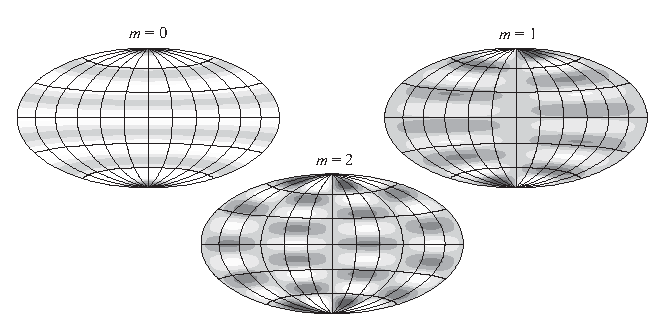
\includegraphics{../figures/chap10/fig02.eps}
\end{center}
\caption[black&white]{\label{10.fig.blackwhite}
对位于北极的三个"标准"矩张量源的标量响应~$A(\Theta,\Phi)$~的示意图。
({\em 左上图\/})~$M_{rr}$~或~$M_{\theta\theta}+M_{\phi\phi}$~源。
({\em 右上图\/})~$M_{r\theta}$~或~$M_{r\phi}$~(垂直倾滑)源。
({\em 中下图\/})~$M_{\theta\theta}-M_{\phi\phi}$~或~$M_{\theta\phi}$~(垂直走滑)源。
它们分别展示振幅随方位角的各向同性、二极和四极变化花样。
任何这样的高次模式($l=10$)沿纵向的节点数目比沿方位角方向多很多。
地图用Aitoff等面积投影绘制,并叠加了一系列经纬度网格线。
对球型振荡,可以想象当浅色部分向上运动时,深色部分则向下运动,反之亦然。}
\end{figure}

图~\ref{10.fig.blackwhite}显示了径向激发振幅~$A(\Theta,\Phi)$~的特征。
一个~$M_{rr}$~或~$M_{\theta\theta}+M_{\phi\phi}$~源沿方位角方向在~$0\leq \Phi\leq 2\pi$ ~范围内没有节点,而沿纵向在~$0<\Theta<\pi$~范围内则有~$l$~个节点;
一个~$M_{r\theta}$~或~$M_{r\phi}$~(垂直倾滑)源沿方位角方向在~$0\leq \Phi\leq 2\pi$ ~范围内有两个节点,而沿纵向在~$0<\Theta<\pi$~范围内则有~$l-1$~个节点;
最后,一个~$M_{\theta\theta}-M_{\phi\phi}$~或~$M_{\theta\phi}$~(垂直走滑)源沿方位角方向在 ~$0\leq \Phi\leq 2\pi$~范围内有四个节点,而沿纵向在~$0<\Theta<\pi$~范围内则有~$l-2$ ~个节点。
一个一般的源$M_{rr},M_{\theta\theta},M_{\phi\phi}, M_{r\theta},M_{r\phi},M_{\theta\phi}$ 会表现出一个包含这三种“标准”花样的混合图像。
环型振荡显然没有径向的~$\brh$~分量;但要注意的是,它们却是拥有纵向的~$\bThetah$~和横向 的~$\bPhih$~两个分量。球对称地球的球型振荡在地震仪的三个分量上都可以观测到。
对于球谐次数~$l\gg 2$~的模式,(\ref{10.Dexpl2})~式中的纵向导数~$\p_{\Theta}$~会明显大于~$(\sin\Theta)^{-1}\p_{\Phi}$,除了在震源~$\Theta=0$~及其对跖点~$\Theta=\pi$~附近。
\index{antipode}%
因此,高次的环型振荡一般会在横向分量上最为明显,
而高次的球型振荡则会在径向和纵向分量上最为明显。\vspace{-0.5mm}

正如我们在第5.4.6节中所指出的,
浅源地震震源机制的确定是个疑难问题。
\index{source!shallow-focus}%
\index{source!problematical}%
随着震源深度~$h=a-r_{\rm s}$~趋近于零,自由表面边界条件~(\ref{8.bcneed})~要求
\eq \label{10.bcneed}
\dot{V}_{\rm s}-r_{\rm s}^{-1}V_{\rm s}+kr_{\rm s}^{-1}U_{\rm s}
\rightarrow 0,\qquad\dot{W}_{\rm s}-r_{\rm s}^{-1}W_{\rm s}
\rightarrow 0,
\en
\eq
(\kappa_{\rm s}+\fourthirds\mu_{\rm s})\dot{U}_{\rm s}
+(\kappa_{\rm s}-\twothirds\mu_{\rm s})r_{\rm s}^{-1}(2U_{\rm s}-kV_{\rm s})
\rightarrow 0,
\en
因此,一个浅源的~$M_{r\theta}$~或
~$M_{r\phi}$~(垂直倾滑)震源或是一个有以下特点的浅源
\eq
M_{rr}=\left(\frac{\kappa_{\rm s}+\fourthirds\mu_{\rm s}}
{\kappa_{\rm s}-\twothirds\mu_{\rm s}}\right)M_{\theta\theta}
=\left(\frac{\kappa_{\rm s}+\fourthirds\mu_{\rm s}}
{\kappa_{\rm s}-\twothirds\mu_{\rm s}}\right)M_{\phi\phi}
\en
不会激发任何球型或环型振荡。
对震源施加各向异性成分为零的约束:
\eq
M_{rr}+M_{\theta\theta}+M_{\phi\phi}=0
\en
一般可以消除$M_{rr}$~和~$M_{\theta\theta}+M_{\phi\phi}$~的不可确定性。
此时公式~(\ref{10.isorad})~成为
~$A_0=M_{rr}[\dot{U}_{\rm s}-r_{\rm s}^{-1}(U_{\rm s}-\half kV_{\rm s})]$。
\index{moment-tensor response!spherical Earth|)}%
\index{response!spherical Earth|)}%

\renewcommand{\thesection}{$\!\!\!\raise1.3ex\hbox{$\star$}\!\!$
\arabic{chapter}.\arabic{section}}
%\section{Seismometer Response}
\section{地震仪响应}
\index{seismometer response|(}%
\index{seismometer!response of|(}%
\index{response!seismometer|(}%
\label{10.sec.seismo.res}
\renewcommand{\thesection}{\arabic{chapter}.\arabic{section}}

\begin{table}[!t]
\centering
\begin{tabular}{|l|c|rrr|rrr|} \hline
& & & & & & & \\
模式 & 
$\displaystyle{{\raisebox{-1.0ex}{\rm 频率}}\atop{\raisebox{1.0ex}{\rm (毫赫兹)}}}$ &
$\displaystyle{\frac{U}{U_{\hspace{-0.2 mm}\star}}}$\hspace{2.0 mm} &
$\displaystyle{\frac{U_{\rm free}}{U_{\hspace{-0.2 mm}\star}}}$\hspace{1.0 mm} &
$\displaystyle{\frac{U_{\rm pot}}{U_{\hspace{-0.2 mm}\star}}}$\hspace{1.0 mm} &
$\displaystyle{\frac{V}{V_{\hspace{-0.3 mm}\star}}}$\hspace{3.0 mm} &
$\displaystyle{\frac{V_{\rm tilt}}{V_{\hspace{-0.3 mm}\star}}}$\hspace{2.0 mm} &
$\displaystyle{\frac{V_{\rm pot}}{V_{\hspace{-0.3 mm}\star}}}$\hspace{2.0 mm} \\
& & & & & & & \\ \hline
& & & & & & & \\
$\hspace{1.5 mm}{}_{0}{\rm S}_{2}$ & 0.3093 & 0.812 & 0.664 & $-0.476$ & $-0.121$ & 2.148 & $-1.027$ \\
$\hspace{1.5 mm}{}_{0}{\rm S}_{3}$ & 0.4686 & 0.870 & 0.310 & $-0.180$ & 0.502 & 0.701 & $-0.203$ \\
$\hspace{1.5 mm}{}_{0}{\rm S}_{4}$ & 0.6471 & 0.914 & 0.171 & $-0.084$ & 0.672 & 0.408 & $-0.080$ \\
$\hspace{1.5 mm}{}_{0}{\rm S}_{5}$ & 0.8404 & 0.941 & 0.104 & $-0.045$ & 0.760 & 0.280 & $-0.040$ \\
$\hspace{1.5 mm}{}_{0}{\rm S}_{6}$ & 1.0382 & 0.957 & 0.069 & $-0.027$ & 0.810 & 0.214 & $-0.024$ \\
$\hspace{1.5 mm}{}_{0}{\rm S}_{7}$ & 1.2318 & 0.968 & 0.050 & $-0.018$ & 0.839 & 0.177 & $-0.016$ \\
$\hspace{1.5 mm}{}_{0}{\rm S}_{8}$ & 1.4135 & 0.975 & 0.038 & $-0.013$ & 0.855 & 0.156 & $-0.012$ \\
$\hspace{1.5 mm}{}_{0}{\rm S}_{9}$ & 1.5783 & 0.979 & 0.031 & $-0.010$ & 0.865 & 0.145 & $-0.009$ \\
$\hspace{1.5 mm}{}_{0}{\rm S}_{10}$ & 1.7265 & 0.983 & 0.026 & $-0.008$ & 0.870 & 0.138 & $-0.008$ \\
& & & & & & & \\
$\hspace{1.5 mm}{}_{1}{\rm S}_{1}$ & 0.0513 & 0.032 & 0.960 & 0.008 & $-0.028$ & 1.019 & 0.009 \\
$\hspace{1.5 mm}{}_{1}{\rm S}_{2}$ & 0.6799 & 1.032 & 0.175 & $-0.207$ & 1.009 & $-0.041$ & 0.032 \\
$\hspace{1.5 mm}{}_{1}{\rm S}_{3}$ & 0.9398 & 0.991 & 0.088 & $-0.078$ & 1.034 & $-0.061$ & 0.027 \\
$\hspace{1.5 mm}{}_{1}{\rm S}_{4}$ & 1.1729 & 0.985 & 0.056 & $-0.041$ & 1.061 & $-0.086$ & 0.025 \\
$\hspace{1.5 mm}{}_{1}{\rm S}_{5}$ & 1.3703 & 0.983 & 0.041 & $-0.024$ & 1.141 & $-0.176$ & 0.034 \\
$\hspace{1.5 mm}{}_{1}{\rm S}_{6}$ & 1.5220 & 0.982 & 0.033 & $-0.016$
      & ---\hspace{2.0 mm} & ---\hspace{2.0 mm} & ---\hspace{2.0 mm} \\
$\hspace{1.5 mm}{}_{1}{\rm S}_{7}$ & 1.6555 & 0.984 & 0.028 & $-0.012$ & 0.694 & 0.342 & $-0.036$ \\
$\hspace{1.5 mm}{}_{1}{\rm S}_{8}$ & 1.7993 & 0.986 & 0.024 & $-0.009$ & 0.770 & 0.252 & $-0.022$ \\
& & & & & & & \\
$\hspace{1.5 mm}{}_{2}{\rm S}_{3}$ & 1.2422 & 0.949 & 0.048 & 0.003 & 0.963 & 0.036 & 0.001 \\
& & & & & & & \\
$\hspace{1.5 mm}{}_{3}{\rm S}_{1}$ & 0.9439 & 0.919 & 0.081 & 0.000 & 0.953 & 0.047 & 0.000 \\
$\hspace{1.5 mm}{}_{3}{\rm S}_{2}$ & 1.1062 & 0.938 & 0.060 & 0.003 & 0.959 & 0.040 & 0.001 \\
$\hspace{1.5 mm}{}_{3}{\rm S}_{8}$ & 2.8196 & 0.988 & 0.010 & 0.002 & 0.990 & 0.010 & 0.001 \\
& & & & & & & \\ \hline
\end{tabular}
\caption[accelresponse]
{惯性、自由空气、倾斜和势函数微扰对一些有代表性的球型振荡的加速度响应算子~$\bD_{\star}$ 
~的贡献的相对大小。
表中所列的数值是横向各向同性PREM模型的结果。
第二列是相应的本征频率~$\omega/2\pi$,单位为毫赫兹。
模式~${}_1{\rm S}_6$~不太可能在水平偏振的仪器上观察到,因为它的~$V\ll U$。}
\label{10.table}
\end{table}
\index{accelerometer}%
正如我们在第4.4节中所看到的,加速度仪除了会对仪器外壳本身的加速度~$\p_t^2\bs$~响应之外,
也会对地球引力场的变化有所响应。
这些效应可通过将~(\ref{4.seismo6})~专用于球对称地球来加以考虑。
我们将注意力局限于地震仪位于地表~$r=a$~的惯常情况,
并且利用外部引力梯度公式 $\dot{g}=-2a^{-1}g$。
这样,(\ref{10.Dexpl2})~式中的球型本征函数需要做
~$U\rightarrow U+\om^{-2}[2a^{-1}gU+(l+1)a^{-1}P]$~和
~$V\rightarrow V-\om^{-2}(ka^{-1}gU+ka^{-1}P)$~两个替换。
环型振荡当然不会受到影响。
我们用星号来标记进行引力修改后的球型本征函数,将~(\ref{10.vectamp})~式中的~$\bD$ ~以修改后位移算子取代:
\eqa \label{10.Dstar}
\lefteqn{\bD_{\star}=\brh\,U_{\hspace{-0.2 mm}\star}+
\bThetah\,\sqL^{-1}[V_{\hspace{-0.3 mm}\star}\p_{\Theta}
+W(\sin\Theta)^{-1}\p_{\Phi}]} \nonumber \\
&&\mbox{}+\bPhih\,\sqL^{-1}
[V_{\hspace{-0.3 mm}\star}(\sin\Theta)^{-1}\p_{\Phi}-W\p_{\Theta}],
\ena
其中
\eqa \label{10.gravterms1} \lefteqn{
U_{\hspace{-0.2 mm}\star}=U+U_{\rm free}+U_{\rm pot},\qquad
U_{\rm free}=2\om^{-2}ga^{-1}U,} \nonumber \\
&&\mbox{}U_{\rm pot}=(l+1)\om^{-2}a^{-1}P,
\ena
\eqa \label{10.gravterms2} \lefteqn{
V_{\hspace{-0.3 mm}\star}=V+V_{\rm tilt}+V_{\rm pot},\qquad
V_{\rm tilt}=-k\om^{-2}ga^{-1}U,} \nonumber \\
&&\mbox{}V_{\rm pot}=-k\om^{-2}a^{-1}P.
\ena
$U_{\rm free}$~和~$V_{\rm tilt}$~两项分别来自地震仪的径向位移所引起的
自由空气引力的变化和无法分辨的地面倾斜与水平加速度,
\index{free-air correction}%
\index{tilt correction}%
而~$U_{\rm pot}$~和~$V_{\rm pot}$~两项则源于地球质量重新分布而造成的引力势函数微扰~$P$。
表~10.1~就一些球型振荡列举了~(\ref{10.gravterms1})--(\ref{10.gravterms2})~中各项的相对大小。
对所有的高频模式,$\om^2\gg\ ga^{-1}$~和~$P\ll gU$,因而$U_{\hspace{-0.2 mm}\star}\approx U$~和~$V_{\hspace{-0.3 mm}\star}\approx V$。
自由空气效应~$U_{\rm free}$~和倾斜~$V_{\rm tilt}$~主导了Slichter
模式${}_1{\rm S}_1$的响应,
\index{Slichter mode}%
\index{mode!Slichter}%
对如~${}_0{\rm S}_2$~这些基阶低次模式的响应也有明显的贡献。
引力势函数微扰~$U_{\rm pot},V_{\rm pot}$~对基阶低次模式也很重要。
而令人惊讶的是,倾斜效应~$V_{\rm tilt}$~即使对中等频率的~${}_0{\rm S}_l$~和~${}_1{\rm S}_l$~模式也是不可忽略的。
一般来讲,这些自引力修正很容易做,
因此在计算合成地震图和频谱时,最好能够常规的使用~$\bD_{\star}$~而不是~$\bD$。

%\section{Wiggly Lines---At Last!}
\section{终于看到波浪线了!}
\label{wiggly}
经过区区~\pageref{wiggly}页,我们终于汇集了在球对称、无自转、微弱非弹性的地球上用模式叠加计算合成地震图所需要的工具。
在本节中我们会展示一些具代表性的加速度频谱、时间域加速度和位移地震图的范例,
并描述其主要特征。
我们不会详述每条记录中的每一个波形起伏,
而是以"一图胜千言"这句格言为宗旨。我们的目的仅仅是用几个可见的范例来展示模式叠加
合成地震图的丰富性和完备性。
作为本章中印象式描述的补充,我们将在第~11~章和第~12~章分别对勒夫与瑞利面波和P-SV体
波做更延伸性的讨论。

%\subsection{Computational details}
\subsection{计算细节}

下面我们将一步一步的描述计算合成加速度图和频谱的习惯步骤。
\index{accelerogram}%
\index{accelerometer!polarization of}%
\index{synthetic accelerogram}%
我们用单位矢量~$\bnuh$~表示加速度仪的{\em 偏振\/},一般是径向~($\bnuh=\brh$)、纵向 ~($\bnuh=\bThetah$)~或横向~$(\bnuh=\bPhih$)。

\begin{enumerate}
\item 用~(\ref{10.appacc})~式,在等间隔时间点~$t=n\hspace{0.3 mm}\Delta t$, $n=0,1,2,\ldots$~计算对脉冲矩率张量~$\dot{\bM}(t)=\sqrt{2}M_0\hat{\bM}\,\delta(t)$~的时间域响应,$\Delta t$~是选定的数字化间隔。

\item 对有限时长震源$\dot{\bM}(t)=\sqrt{2}M_0\hat{\bM}\,\dot{m}(t)$的响应
可以通过~(\ref{10.appacc})~式与震源时间函数~$\dot{m}(t)$~的卷积而得到。
在实际中,更简单的做法是将公式~(\ref{10.isorad})--(\ref{10.B2need})~中的矩张量~$\bM$~换成 ~$\sqrt{2}M_0\hat{\bM}\,m(\om)$,其中~$\om$~是~${}_n\om_l^{\rm T}$~或~${}_n\om_l^{\rm S}$,$m(\om)$~是~$\dot{m}(t)$~的傅里叶变换。
为了减少模式叠加的硬性截断所引起的“振荡”及其它非因果的假讯号,
我们一般采用半持续时间为~$\tau_{\rm h}=10.5$~秒的对称矩形震源时间函数 ~$\dot{m}(t)=(2\tau_{\rm h})^{-1}[H(t+\tau_{\rm h})
-H(t-\tau_{\rm h})]$。
\index{source time function}%
这时的傅里叶变换成为一个“辛克”函数~$m(\om)=(\omega\tau_{\rm h})^{-1}\sin(\omega\tau_{\rm h})$。要注意归一化条件:$\int_{-\tau_{\rm h}}^{\tau_{\rm h}}\dot{m}(t)\,dt=1$。

\item  在所有范例中,用~(\ref{10.Dstar})~式中的修改后位移算子~$\bD_{\star}$~对
自由空气、倾斜和势函数微扰对加速度仪的影响加以考虑。

\item 采用时间到频率的离散傅里叶变换来计算频谱~$\bnuh\cdot\ba(\bx,\om)$,而不是借由公式~(\ref{10.accfreq})~直接在频率域计算。将时间域记录~$\bnuh\cdot\ba(\bx,t)$~想要的部分分离出来,
并乘以~Hann~或余弦钟形时窗函数(两端平滑衰减)以减少因模式之间的干涉而导致的频谱漏失和谱峰失真效应 (Harris \citeyear{harris78}; Dahlen \citeyear{dahlen82})。
如果选取的时窗段包含时间为~$t=n\hspace{0.3 mm}\Delta t$, $n=0,1,\ldots,N-1$~的~$N$~个采样点,
则~Hann~钟形函数对应的权重为~$w_n=w(n\hspace{0.3 mm}\Delta t)=
\half\{1-\cos[2\pi n/(N-1)]\}$。
在进行快速傅里叶变换之前,对钟形函数时间序列在~$t=(N-1)\Delta t$ ~点之后补零。这样做的效果是在相邻傅里叶频率~$\omega_n=(2\pi n)/(N\hspace{0.3 mm}\Delta t)$,
$n=-N\hspace{-0.2 mm}/2,\ldots,N\hspace{-0.2 mm}/2$~之间对频谱进行内插。
\end{enumerate}

除非另行说明,我们在计算合成地震图和频谱中叠加了周期为~8~秒或更长的所有地幔环型模式~${}_n{\rm T}_l$
~和球型模式~${}_n{\rm S}_l$。总计有~60,000~多个环型和~100,000~多个球形振荡模式。
我们用来构建本征频率-本征函数目录的球对称地球模型是横向各向同性的~PREM。
为了展示的目的,我们一般画出的是被称为{\em 振幅谱}的绝对值~$|\bnuh\cdot\ba(\bx,\omega)|$。
\index{spectrum!amplitude}%
\index{amplitude spectrum}%
也可能会画出{\em 功率谱},即绝对值的平方~$|\bnuh\cdot\ba(\bx,\omega)|^2$。
\index{spectrum!power}%
\index{power spectrum}%

%\subsection{Spectra}
\subsection{频谱}
\index{spectrum|(}%

我们首先考虑一个假想的浅源逆冲地震的频谱或频率域响应;
断层面的走向为北~$45^{\circ}$~西,倾角为东北~$45^{\circ}$;
矩张量点源的深度为~33~公里。
图~\ref{fig:10.3}显示了该地震正东方、震中距~$\Theta=60^\circ$ ~处的横向分量振幅谱~$|\bPhih\cdot\ba(\bx,\omega)|$。
\begin{figure}
\begin{center}
\scalebox{0.97}{
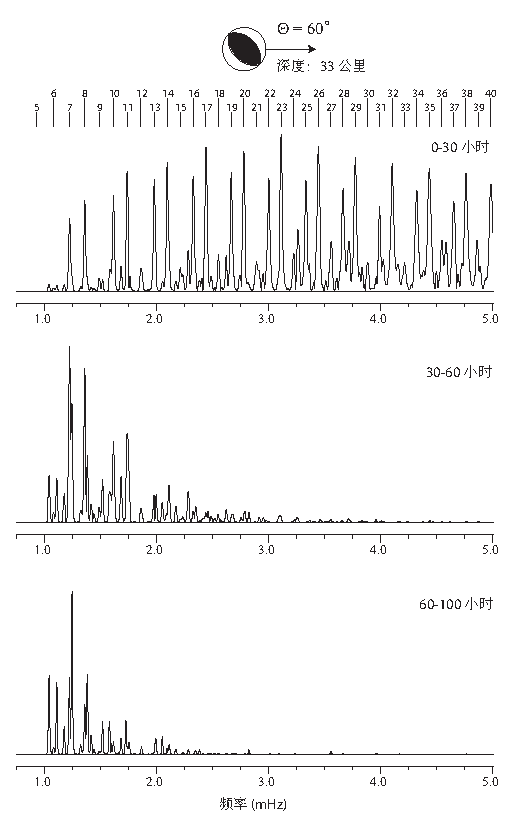
\includegraphics{../figures/chap10/fig03.eps}
}
\end{center}
\caption[thrust spect1]{
\label{fig:10.3}
PREM地球模型中假想的浅源逆冲断层的横向分量合成加速度谱。
({\em 上图\/}) $t=0\hspace{0.2 mm}$--$\hspace{0.2 mm}30$
小时; 
({\em 中图\/}) $t=30\hspace{0.2 mm}$--$\hspace{0.2 mm}60$
小时; 
({\em 下图\/}) $t=60\hspace{0.2 mm}$--$\hspace{0.2 mm}100$
小时。
中下图中两个经过衰减过滤的频谱的最大振幅分别减小为上图中未经衰减过滤频谱的最大振幅的~0.056~和~0.013。
最顶部为震源机制和接收点方位示意图;
沙滩球上的黑色和白色区域分别对应于下半震源球上~P~波压缩和扩张的象限。
环型基阶模式~${}_0{\rm T}_5$~至~${}_0{\rm T}_{40}$~的位置以垂直线表示。相应的径向分量见图~\protect\ref{fig:10.5}。}
\end{figure}
\begin{figure}
\begin{center}
\scalebox{0.9}{
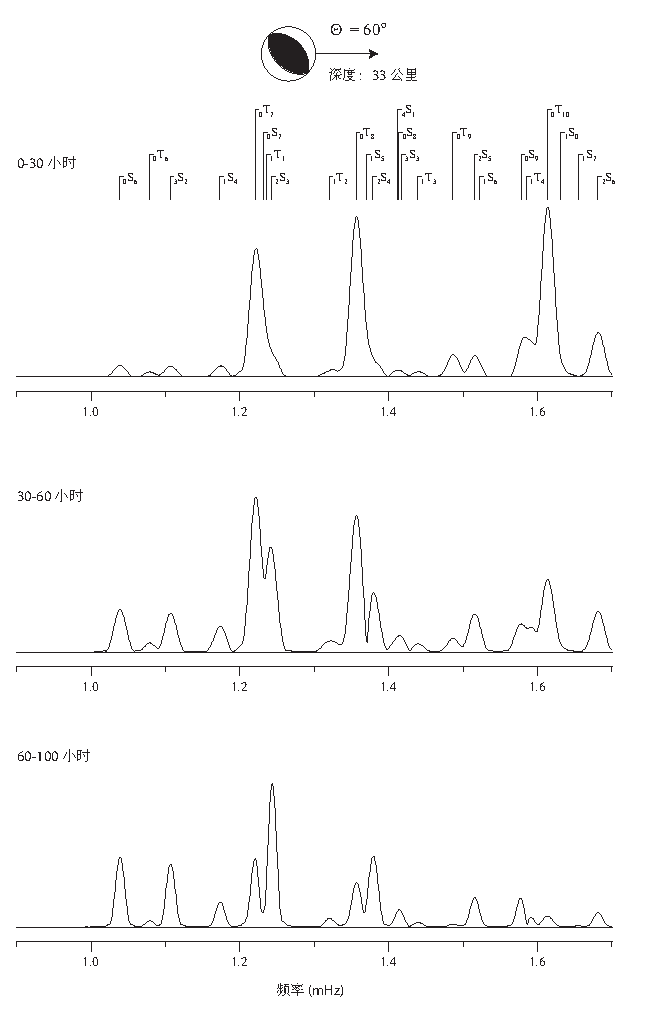
\includegraphics{../figures/chap10/fig04.eps}
}
\end{center}
\caption[thrust zoom1]{
\label{fig:10.4}
图~\protect\ref{fig:10.3}的低频部分放大图。
中下图中两个经过衰减过滤的频谱的最大振幅分别减小为上图中未经衰减过滤频谱的最大振幅的~0.092~和~0.021。
图的顶部标示了一些频谱中可见的环型和球型模式。
相应的径向分量见图~\protect\ref{fig:10.6}。}
\end{figure}
\begin{figure}
\begin{center}
\scalebox{0.97}{
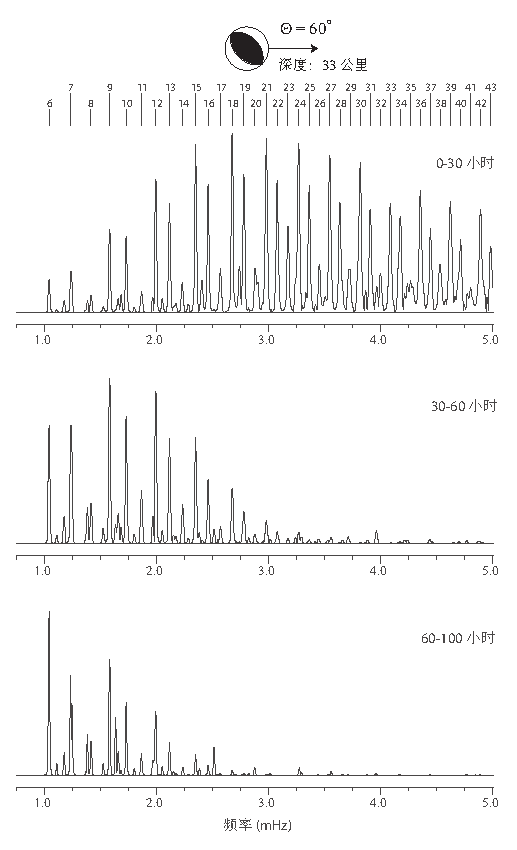
\includegraphics{../figures/chap10/fig05.eps}
}
\end{center}
\caption[thrust spect2]{
\label{fig:10.5}
PREM地球模型中假想的浅源逆冲断层的径向分量合成加速度谱。
({\em 上图\/}) $t=0\hspace{0.2 mm}$--$\hspace{0.2 mm}30$
小时; 
({\em 中图\/}) $t=30\hspace{0.2 mm}$--$\hspace{0.2 mm}60$
小时; ({\em 下图\/}) $t=60\hspace{0.2 mm}$--$\hspace{0.2 mm}100$
小时。
中下图中两个经过衰减过滤的频谱的最大振幅分别减小为上图中未经衰减过滤频谱的最大振幅的~0.093~和~0.027。
最顶部为震源机制和接收点方位示意图;
沙滩球上的黑色和白色区域分别对应于下半震源球上~P~波压缩和扩张的象限。
球型基阶模式~${}_0{\rm S}_6$~至~${}_0{\rm S}_{43}$~的位置以垂直线表示。相应的横向分量见图~\protect\ref{fig:10.3}。}
\end{figure}
\begin{figure}
\begin{center}
\scalebox{0.96}{
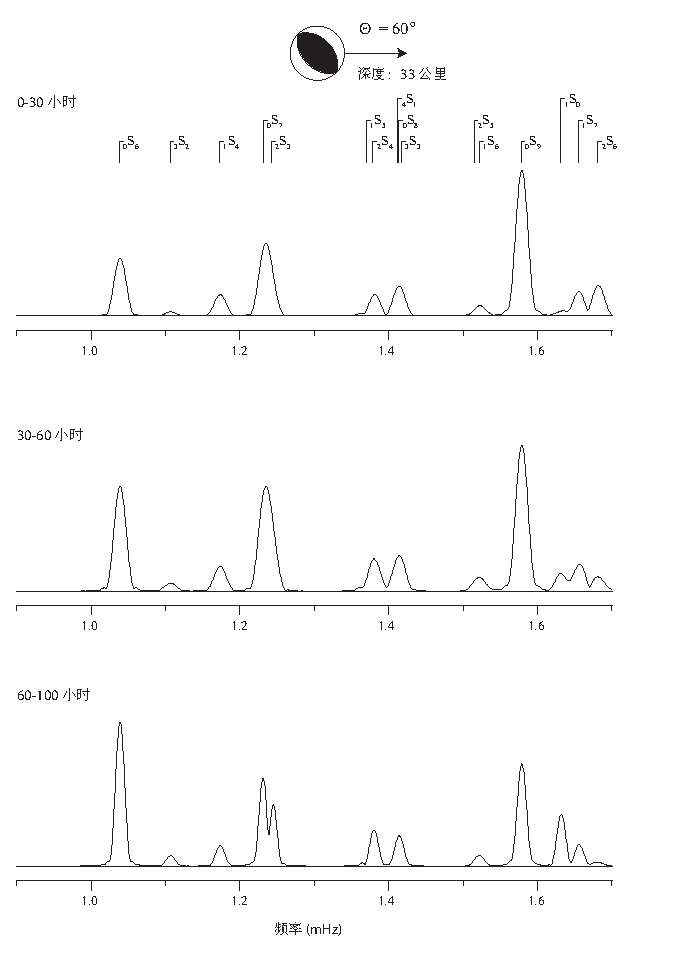
\includegraphics{../figures/chap10/fig06.eps}
}
\end{center}
\caption[thrust zoom2]{
\label{fig:10.6}
图~\protect\ref{fig:10.5}的低频部分放大图。
中下图中两个经过衰减过滤的频谱的最大振幅分别减小为上图中未经衰减过滤频谱的最大振幅的~0.200~和~0.059。
图的顶部标示了一些频谱中可见的球型模式。
相应的横向分量见图~\protect\ref{fig:10.4}。}
\end{figure}
\begin{figure}
\begin{center}
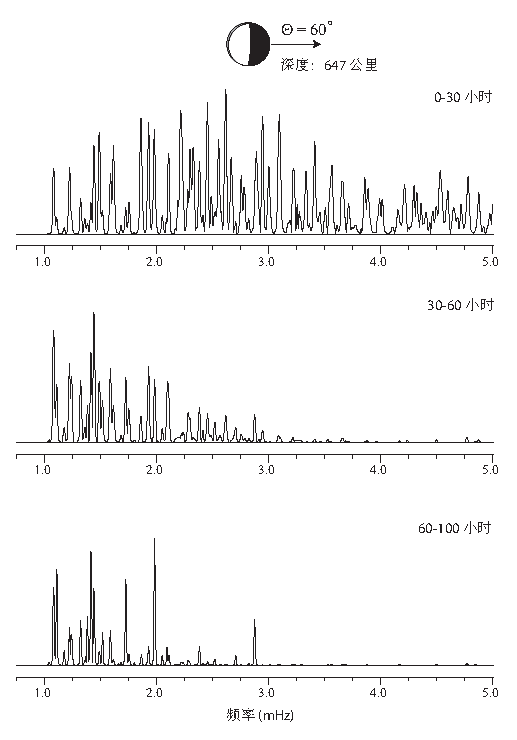
\includegraphics{../figures/chap10/fig07.eps}
\end{center}
\caption[Bolivia spect1]{
\label{fig:10.7}
1994年6月9日玻利维亚深源地震的横向分量合成加速度谱。
({\em 上图\/}) $t=0\hspace{0.2 mm}$--$\hspace{0.2 mm}30$
小时; 
({\em 中图\/}) $t=30\hspace{0.2 mm}$--$\hspace{0.2 mm}60$
小时;  
({\em 下图\/}) $t=60\hspace{0.2 mm}$--$\hspace{0.2 mm}100$
小时。 
中下图中两个经过衰减过滤的频谱的最大振幅分别减小为上图中未经衰减过滤频谱的最大振幅的~0.089~和~0.022。
最顶部带箭头的沙滩球显示了接收点方位与地震震源机制之间的关系;
为显示方便,将该沙滩球逆时针旋转了约~$90^\circ$。玻利维亚地震震源机制解的正确方向显示在图\ref{fig:10.20}中;接收点位于南方。相应的径向分量见图~\protect\ref{fig:10.9}。}
\end{figure}
\begin{figure}
\begin{center}
\scalebox{0.92}{
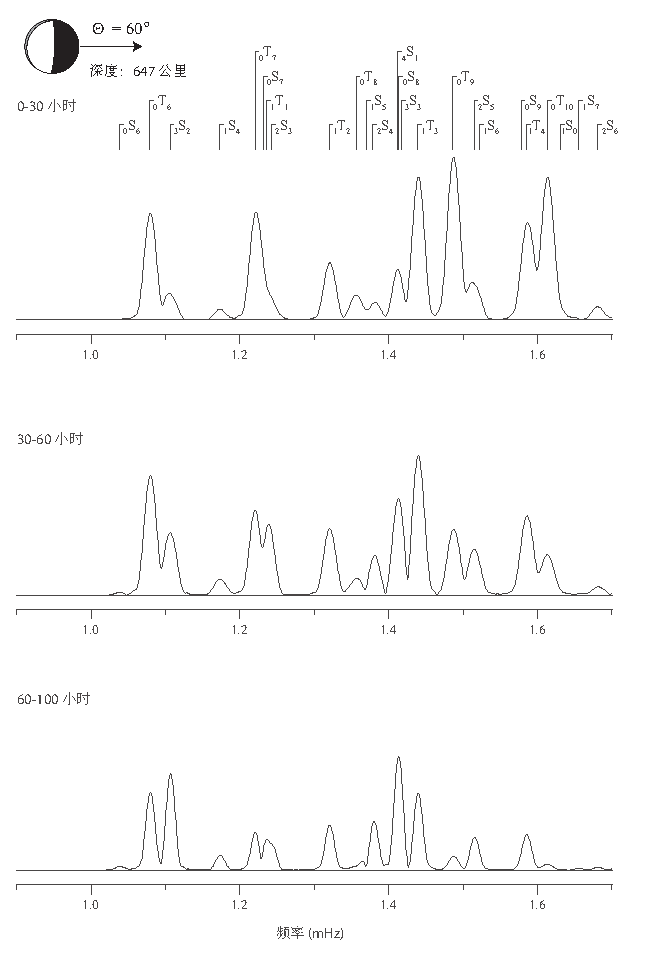
\includegraphics{../figures/chap10/fig08.eps}
}
\end{center}
\caption[Bolivia zoom1]{
\label{fig:10.8}
图~\protect\ref{fig:10.7}低频部分的放大图。
中下图中两个经过衰减过滤的频谱的最大振幅分别减小为上图中未经衰减过滤频谱的最大振幅的~0.128~和~0.028。
图的顶部标示了一些频谱中可见的环型和球型模式。}
\end{figure}
最上面一幅图中的频谱是将模式叠加得到的加速度图~$\bPhih\cdot\ba(\bx,t)$~中从发震时刻~$t=0$~至~$t=30$~小时的一段截取出来,然后乘以~Hann~钟形函数而得到。
在~1--5~毫赫兹频段中最显著的谱峰所对应的是~${}_0{\rm T}_5$~至~${}_0{\rm T}_{40}$~的基阶环型振荡。
顶部标示了这些被强烈激发模式的理论本征频率;
最大频谱振幅出现在~3.11~毫赫兹,对应于模式~${}_0{\rm T}_{23}$。
中间一幅图的频谱是将加速度图的~$t=30$~小时至~$t=60$~小时一段截取出来,再乘以~Hann~钟形函数而得到。这一直接舍弃数据而重新计算频谱的过程被称为{\em 衰减过滤\/}。
\index{attenuation filtering}%
$Q$~值相对较低的模式,即这里的频率较高的基阶模式,往往在过滤后的频谱中被消除;剩下的最高谱峰对应于模式~${}_0{\rm T}_7$。
在最下面一幅图中的频谱是将加速度图的~$t=60$~小时至~$t=90$~小时一段截取出来,再乘以~Hann~钟形函数而得到,剩下的~$Q$~值较高的模式数目更少;
请注意,这是从地震发生后两天半到四天的时段。

在图~\ref{fig:10.4}中,我们将图~\ref{fig:10.3}中~0.9~至~1.7~毫赫兹 之间的低频部分放大,以便进一步探究衰减过滤的影响。
在顶部标示了该频率范围内值得关注的环型和球型振荡。
以天真的射线理论观点(仅当~$\omega\rightarrow\infty$~时才严格成立),
我们不应当期望在加速度仪的横向分量上看到球型模式。
而事实上,我们看到一些长周期、高~$Q$~值的球型模式实际上主导了~60--100~小时的频谱!
其中最高的谱峰是~${}_2{\rm S}_3$~这个径向二阶模式,在地震发生~30~个小时之后在基阶环型模式 ~${}_0{\rm T}_7$~的高频一侧的斜坡上显露出来。
模式~${}_0{\rm S}_6$、${}_3{\rm S}_2$、${}_1{\rm S}_4$~和~${}_2{\rm S}_4$~也都是在发震~60~小时之后变得明显。

图~\ref{fig:10.5}显示了来自同一源点-接收点组合的径向分量频谱~$|\brh\cdot\ba(\bx,\omega)|$。
0--30~小时频谱中主导的谱峰是~${}_0{\rm S}_6$~至~${}_0{\rm S}_{43}$~的基阶球型振荡,标示在顶部。
在未经衰减过滤的横向分量频谱中,振幅最大的~${}_0{\rm S}_{18}$
~比~${}_0{\rm T}_{23}$~大一倍半。
在舍弃前~30~小时或前~60~小时的数据后,高频、低~$Q$~值的基阶模式仍然会被消除。
图~\ref{fig:10.6}展示了~0.9~和~1.7~毫赫兹之间的衰减过滤前后的频谱放大图。
值得注意的是,出现在衰减过滤后横向频谱中的许多低频球型模式在过滤后的径向频谱中也占主导地位。
还有一个明显的新的谱峰,即一阶径向模式~${}_1{\rm S}_0$,
依照定义在水平向的加速度仪上是无法观测到它的。

作为第二个例子,我们来考虑1994年6月9日发生在玻利维亚647公里深处的地震。
\index{Bolivia 1994 earthquake}%
\begin{figure}
\begin{center}
\scalebox{0.91}{
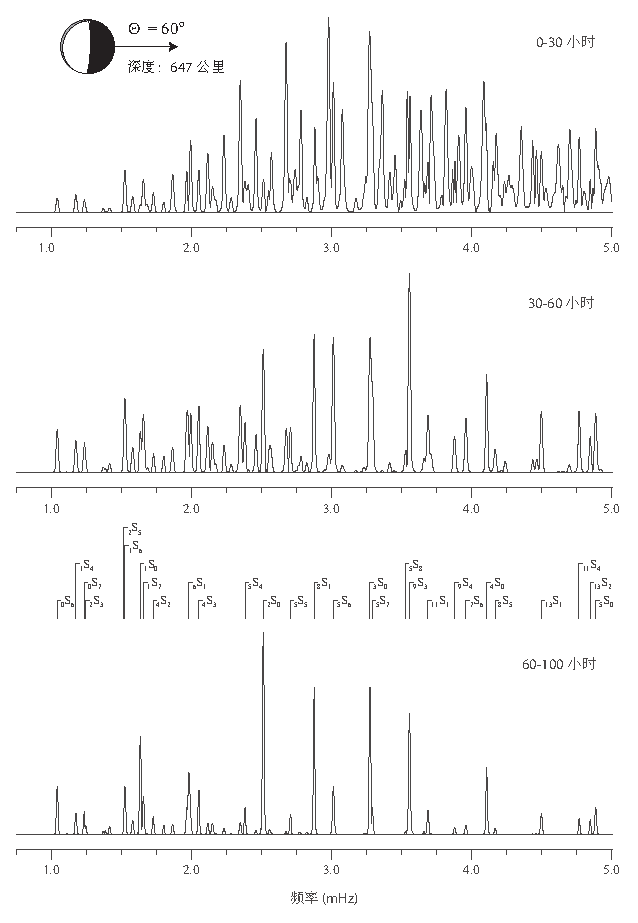
\includegraphics{../figures/chap10/fig09.eps}
}
\end{center}
\caption[Bolivia spect2]{
\label{fig:10.9}
1994年6月9日玻利维亚深源地震的径向分量合成加速度频谱。
({\em 上图\/}) $t=0\hspace{0.2 mm}$--$\hspace{0.2 mm}30$
小时;
({\em 中图\/}) $t=30\hspace{0.2 mm}$--$\hspace{0.2 mm}60$
小时;
({\em 下图\/}) $t=60\hspace{0.2 mm}$--$\hspace{0.2 mm}100$
小时。
中下图中两个经过衰减过滤的频谱的最大振幅分别减小为上图中未经衰减过滤频谱的最大振幅的~0.127~和~0.049。
在最顶部显示了(经旋转的)地震震源机制与接收点方位;
图中标示了在~60-100~小时的频谱中可以看见的一些高~$Q$~值的球型振荡。
相应的横向分量见图~\protect\ref{fig:10.7}。}
\end{figure}
该地震发生在纳斯卡俯冲板块内,地震矩为~$M_0=2.4\times 10^{21}$~牛顿-米,它是迄今为止由现代地震仪所记录到的最大的深源地震。
我们展示在一个位于震源机制的P波压缩象限、震中距为~$\Theta=60^\circ$~的假想台站的一些合成加速度频谱。
图~\ref{fig:10.7}显示了~0--30~小时、30--60~小时和~60--100~小时三个时段的乘以~Hann~钟形函数后的横向分量频谱~$|\bPhih\cdot\ba(\bx,\omega)|$。
和之前一样,一些低频、高~$Q$~值的球型模式在经衰减过滤后的频谱中十分显著;
在~0.9--1.7~毫赫兹频段的放大图~\ref{fig:10.8}中,对这些模式以及掺杂其中的环型模式都做了辨识。

图~\ref{fig:10.9}显示了玻利维亚地震的径向分量合成频谱 $|\brh\cdot\ba(\bx,\omega)|$ 。它与~\ref{fig:10.5}中的浅源地震形
成了鲜明的对比:在舍弃前~30~至前~60~小时的数据后,更多的中等频率和高频的谱
峰依然可见。在最下面一幅图的上方标示了经~60-100~小时的衰减过滤后频谱中仍然可以识别的谱峰。
它们都是高~$Q$~值的~PKIKP~等价的球型模式,包括前五阶径向模式
~${}_1{\rm S}_0\,$--$\,{}_5{\rm S}_0$, 以及其它振荡模式,如~${}_2{\rm S}_3$、${}_8S_1$、
${}_9{\rm S}_3$、${}_{11}{\rm S}_1$、${}_8{\rm S}_5$、
${}_{13}{\rm S}_1$、${}_{11}{\rm S}_4$~和~${}_{13}{\rm S}_2$。
后面这几个是极为有趣的振荡,它们对地球内部最深处的性质有敏感性。
在第~14.2.8~节中,我们将看到这些多态模式因地球自转、流体静力学的椭率以及地幔中大尺度横向不均匀性这些有良好描述的模型微扰所产生的分裂远超出预期的程度。
这种所谓的{\em 异常分裂}为内核的各向异性提供了最初的证据~(Woodhouse,
Giardini \& Li \citeyear{woodhouse&al86}; Tromp \citeyear{tromp93})。
\index{anomalous splitting}%
\index{splitting!anomalous}%
\index{anisotropy!inner-core}%
\index{inner-core anisotropy}%

%\subsection{Seismograms}
\subsection{地震图}
\index{seismogram|(}%
\index{accelerogram|(}%

在图~\ref{fig:10.11}中,我们展示了一些横向分量的合成加速度图~$\bPhih\cdot\ba(\bx,t)$。
这里的假想震源是一个位于~33~公里深处的垂直走滑断层。
如图顶部所示,台站位于该右旋断层的延伸线上,震中距为~$\Theta=30^\circ$、$\Theta=60^\circ$~和~$\Theta=90^\circ$~的地方。
这一几何关系使得只有环型模式~${}_n{\rm T}_l$~会被激发。
对上面的三道记录做了周期~20~至~80~秒的带通滤波,以突显出直达和反射体波讯号。
可以很容易地识别一些明显的震相,如~SH、${\rm SS}_{\rm SH}$、${\rm SSS}_{\rm SH}$~和
~${\rm SKKS}_{\rm SH}$。
对下面的三道记录做了周期~50~至~250~秒的带通滤波,以显示长周期的基阶勒夫波或G波。

\begin{figure}[!b]
\begin{center}
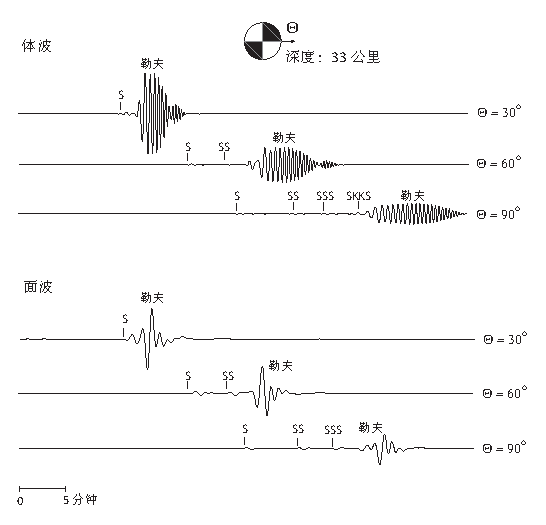
\includegraphics{../figures/chap10/fig10.eps}
\end{center}
\caption[seismogram1]{
\label{fig:10.11}
在一个假想浅源右旋走滑断层正东方震中距为~$\Theta=30^\circ$、$\Theta=60^\circ$~和 ~$\Theta=90^\circ$~处的横向分量合成加速度地震图。
在图的最上方示意性地显示了震源机制和接收点的方位。
({\em 上图\/})周期~20--80~秒带通滤波后的地震图,以凸显~SH~体波讯号。 
({\em 下图\/})周期~50--250~秒带通滤波后的地震图,以凸显勒夫面波。}
\end{figure}

\begin{figure}
\begin{center}
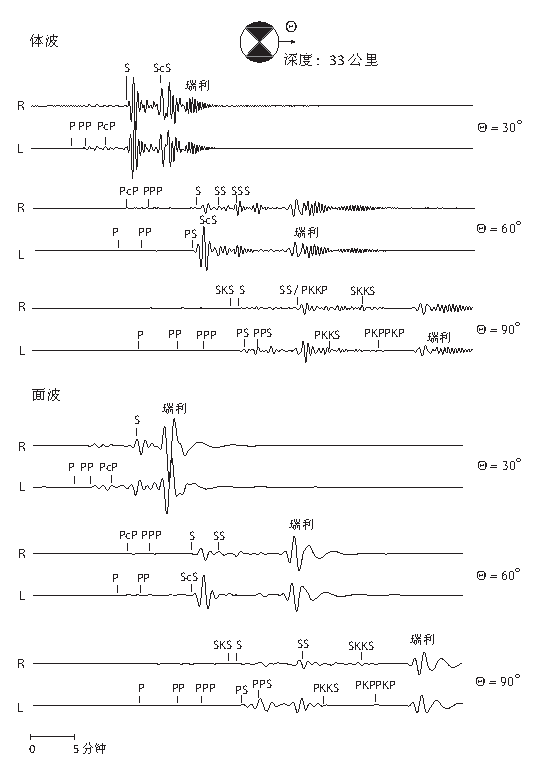
\includegraphics{../figures/chap10/fig11.eps}
\end{center}
\caption[seismogram2]{
\label{fig:10.13}
在一个假想浅源右旋走滑断层正东方震中距为~$\Theta=30^\circ$、$\Theta=60^\circ$~和 ~$\Theta=90^\circ$~处的径向~(R)~和纵向~(L)~分量合成加速度图。
在图的最上方示意性地显示了震源机制和接收点的方位。
({\em 上图\/})周期~20--80~秒带通滤波后的地震图,以凸显出~P~和~SV~体波讯号。 
({\em 下图\/})周期~50--250~秒带通滤波后的地震图,以凸显瑞利面波。
}
\end{figure}
\begin{figure}[!t]
\begin{center}
\scalebox{1.05}{
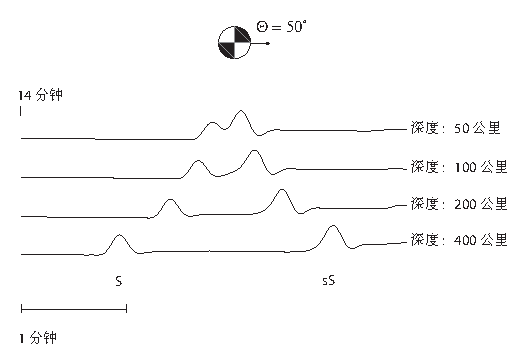
\includegraphics{../figures/chap10/fig12.eps}
}
\end{center}
\caption[seismogram3]{
\label{fig:10.14}
在一个假想右旋走滑断层正东方震中距为~$\Theta=50^\circ$~处的横向分量位移地震图。
在图的最上方示意性地显示了震源机制和接收点的方位。
随着震源深度从~50~公里({\em 最上\/})增加到~400~公里 ({\em 最下\/}),
地表反射震相~${\rm sS}_{\rm SH}$~逐渐“远离”直达震相~SH。}
\end{figure}
\begin{figure}[!t]
\begin{center}
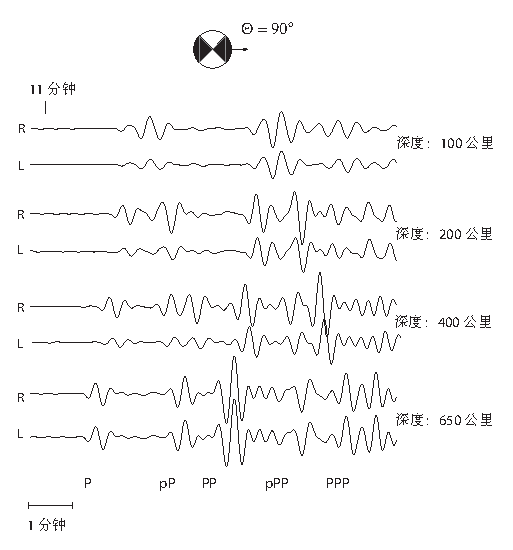
\includegraphics{../figures/chap10/fig13.eps}
\end{center}
\caption[seismogram4]{
\label{fig:10.15}
在一个假想右旋走滑断层正东方震中距为~$\Theta=90^\circ$~处的径向~(R)~和纵向~(L)~合成加速度图,
在图的最上方示意性地显示了震源机制和接收点的方位。
随着震源深度从~100~公里({\em 最上\/})增加到~650~公里 ({\em 最下\/}),
地表反射的“深度震相”~pP~和~ppp~逐渐“远离”直达震相~P~和~PP。}
\end{figure}

图~\ref{fig:10.13} 显示了位于三个震中距~$\Theta=30^\circ$、$\Theta=60^\circ$
~和~$\Theta=90^\circ$~处的径向和纵向加速度图~$\brh\cdot\ba(\bx,t)$~和 ~$\bThetah\cdot\ba(\bx,t)$。震源仍然是深度为~33~公里的垂直走滑断层;
但与前面的例子相比,断层走向旋转了~$45^{\circ}$,因此只有球型模式~${}_n{\rm S}_l$~会被激发。
最上面的六道记录是做了周期~20~至~80~秒滤波的结果,以凸显~P-SV~体波;
值得注意的是,长周期的剪切波震相~(如~SV~和~${\rm ScS}_{\rm SV}$)~比压缩波震相~(如~P~和~PcP)~更加明显。
最下面的六道记录显示同样的加速度图,但做了不同滤波来强调基阶模式瑞利波。
径向和纵向波列的频散特征十分明显:周期~50-100~秒的波明显比~200-250~秒的"地幔"瑞利波早到。
在第~\ref{11.sec.disper}节中我们将更详细地讨论瑞利波和勒夫波的频散。

在图~\ref{fig:10.14}中,我们展示震源深度对最早的两个横向分量体波讯号的影响。
这里所选择的垂直走滑震源机制和接收点方位是使得只有环型模式 ${}_n{\rm T}_l$会被激发; 震中距为$\Theta=50^\circ$。如预期的,随着事件的深度从50公里增加到400公里,
直达SH波到得越来越早,而地表反射震相 ${\rm sS}_{\rm SH}$则到得越来越晚。
图中所展示的是质点位移$\bPhih\cdot\bs(\bx,t)$,而不是加速度 $\bPhih\cdot\ba(\bx,t)$;
同时为了使这一"震相随深度增加而远离"的图像更清楚,采用了半持续时间为$\tau_{\rm h}=10.5$秒的等腰三角形而不是矩形函数来作为震源时间函数$\dot{m}(t)$。
图~\ref{fig:10.15}显示了震源深度对径向和纵向P-SV体波的类似效应。
该台站位于与一个走滑地震的震中距为 $\Theta=90^\circ$的位置上,
其方位使得只有球型模式 ${}_n{\rm S}_l$会被激发。
随着地震事件深度从100 公里增加到650公里,pP--P和~pPP--PP的时间间隔都在增大。
在实际工作中,这些不同的直达与地表反射震相之间的到时差观测,
对地震深度提供了一个重要的约束。
\index{focal depth}%

\begin{figure}[!t]
\begin{center}
\scalebox{0.86}{
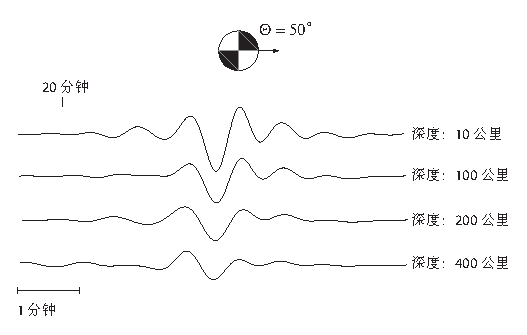
\includegraphics{../figures/chap10/fig14.eps}
}
\end{center}
\caption[seismogram5]{
\label{fig:10.16}
在一个假想右旋走滑断层正东方震中距为~$\Theta=50^\circ$~处的横向分量合成加速度图,
显示勒夫波的振幅随着震源深度从~10~公里~({\em 最上\/})~至~400~公里~({\em 最下\/})~的增加而减小。}
\end{figure}
\begin{figure}[!b]
\begin{center}
\scalebox{0.86}{
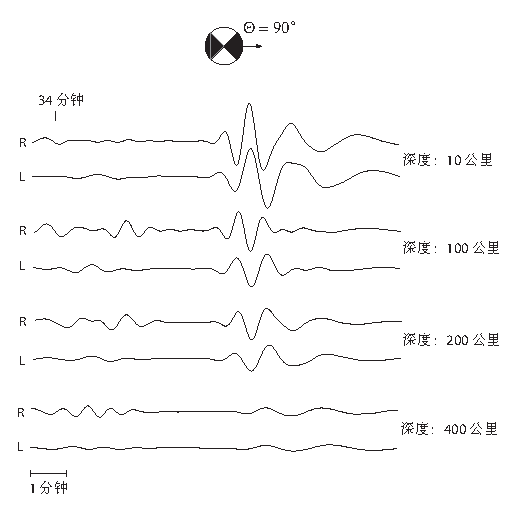
\includegraphics{../figures/chap10/fig15.eps}
}
\end{center}
\caption[seismogram6]{
\label{fig:10.17}
在一个假想右旋走滑断层正东方震中距为~$\Theta=90^\circ$~处的径向~(R)~和纵向~(L)~合成加速度图,
显示瑞利波的振幅随着震源深度从~10~公里~({\em 最上\/})~至~400~公里~({\em 最下\/})~的增加而减小。}
\end{figure}

图~\ref{fig:10.16}和~\ref{fig:10.17}展示了震源深度对基阶模式面波激发的影响。
图中源点-接收点之间的几何关系与图~\ref{fig:10.14}和~\ref{fig:10.15}相同,
因而前一张图中只有勒夫波被激发,而后一张图只有瑞利波被激发。
从径向和纵向分量的比较可以明显看出瑞利波的逆进质点运动特征。
随着走滑地震的深度从~10~公里增加到~400~公里,两种类型的面波振幅都在减小。
深源地震辐射相对较弱的基阶模式地震波,
因为其震源是在相应的~${}_0{\rm T}_l$~和~${}_0{\rm S}_l$~本征函数的准指数衰减的末端,实质上是处于节点的位置。

\begin{figure}[!t]
\begin{center}
\scalebox{0.96}{
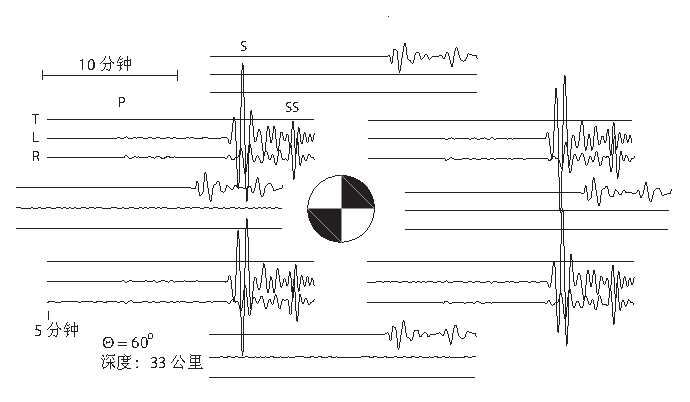
\includegraphics{../figures/chap10/fig16.eps}
}
\end{center}
\caption[seismogram7]{
\label{fig:10.18}
体波辐射花样对合成加速度图的影响。
震源是位于~$h=33$~公里深度的右旋走滑断层;
中央沙滩球中的黑色和白色区域分别对应于下半震源球上~P~波的压缩和扩张象限。
八个三分量地震台站位于(从顶部沿顺时针方向)北方、东北方、东方、东南方、南方、西南方、西方和西北方,震中距均为$\Theta=60^{\circ}$ 。在西北方台站记录上标示了
横向~(T)、纵向~(L)~和径向~(R)~分量以及~P~波、S~波和~SS~波震相。}
\end{figure}
\begin{figure}[!t]
\begin{center}
\scalebox{0.99}{
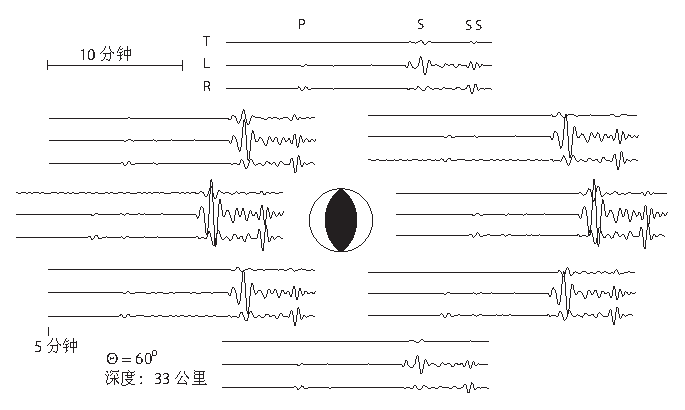
\includegraphics{../figures/chap10/fig17.eps}
}
\end{center}
\caption[seismogram8]{
\label{fig:10.19}
与图~\protect\ref{fig:10.18}相同,但震源为浅源~($h=33$~公里)~逆冲断层。
在位于北方台站的合成加速度图上标示了横向~(T)、纵向~(L)~和径向~(R)~分量以及~P~波、S~波和~SS~波。
所有记录都做了周期~20~到~80~秒的带通滤波,以凸显~P-SV~为主的体波。}
\end{figure}

图~\ref{fig:10.18} 探讨了垂直走滑震源机制对~SH~和~P-SV~体波辐射花样的影响。
每一组三分量加速度图相对于中心沙滩球的位置反映了相应台站相对于地震事件的方位。
这八个三分量台站的震中距均为~$\Theta=60^\circ$;
合成记录都做周期~20-80~秒的带通滤波,以便强化体波。
在图~\ref{fig:10.18}中,位于北、东、南、西四个台站的径向和纵向分量上都没有可见讯号,
这是由于在断层面与辅助面方向都是~P~波和~SV~波的节点。
然而,这四个台站上~SH~波辐射花样的与节点相反的特征,
使得横向分量上有明显的~SH~和~${\rm SS}_{\rm SH}$~讯号。 而东北、东南、西南和西北四个台站的径向和纵向分量上则展现出与节点相反的较强的~P、SV~和~${\rm SS}_{\rm SV}$~讯号,并且在横向分量上看不到~SH~讯号。
图~\ref{fig:10.19}显示了一个南北走向、倾角~$45^{\circ}$~的逆冲断层在相同八个台站的径向、纵向和横向加速度图。
这里最明显的特征是在断层走向的正反两个方向上以纵向偏振为主的剪切波。

在1992年9月2日尼加拉瓜地震发生之后,
\index{Nicaragua 1992 earthquake}%
Kanamori (\citeyear{kanamori93})在一些宽频地震台上观测到P和S波
之间的一个奇怪的长周期波形。
他把这一之前从未注意到的远震讯号归因于远场体波的相长干涉所造成的回音廊效应,
于是称之为{\em W震相\/}。
\index{W phase}%
\index{phase!W}%
这个引起了强烈海啸的尼加拉瓜地震被描述成是在科科斯板块与北美板块之间的俯冲界面上的异常缓慢的破裂(Kanamori \& Kikuchi \citeyear{kanamori&kikuchi93})。
在图~\ref{fig:10.W-phase}中,我们展示了在
帕萨迪纳所观测到的径向位移与利用半持续时间为~$\tau_{\rm h}=40$秒的震源所计算的本征模式合成地震图相当吻合。
Vidale, Goes \& Richards (\citeyear{vidale&al95})指出W震相可以被视为无限均匀介质中以介于$\alpha$ 和$\beta$之间的速度传播、依(距离)$^{-2}$ 和(距离)$^{-3}$而非(距离)$^{-1}$衰减的
中场和近场(Aki \& Richards \citeyear{aki&richards80})能量在球状地球上的表现。
这种非辐射能量无法用我们在第15章中所介绍的射线理论的方法进行
分析;然而,它却完全包含在~(\ref{10.DISPUGLY})式的球对称地球的模式叠加中。

\begin{figure}[!t]
\begin{center}
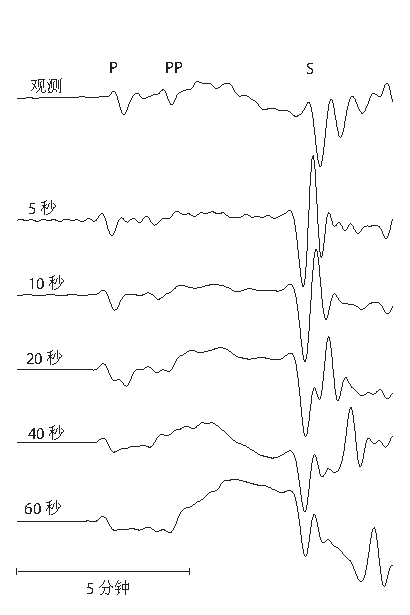
\includegraphics{../figures/chap10/fig18.eps}
\end{center}
\caption[w-phase]{
\label{fig:10.W-phase}
({\em 顶图\/})1992年9月2日尼加拉瓜海啸地震后,在加州帕萨迪纳的宽频台站~PAS~(震中距 ~$\Theta=36.4^{\circ}$)所记录到的径向分量位移地震图~$\hat{\bf r}\cdot{\bf s}({\bf x},t)$ 。
除了标示的~P、PP~和~S~波讯号外,
在~P~和~S~波之间约~$5\!-\!6$~分钟长的时段内到达的还有一个独特的长周期~W~震相。
({\em 下图\/})五个用简正模式叠加得到的径向分量合成地震图;
其中均标出了半持续时间为~$\tau_{\rm h}=5\!-\!60$~秒的震源时间函数~$\dot{m}(t)=(2\tau_{\rm h})^{-1}[H(t+\tau_{\rm h})
-H(t-\tau_{\rm h})]$。
对所有地震图都做了频率~1--30~毫赫兹的巴特沃斯滤波。}
\end{figure}

最后一个---也是我们最喜爱的---例子显示了1994年6月9日玻利维亚深源地震后一个近场位置的
合成质点位移 $\bs(\bx,t)$ (Ekstr\"{o}m \citeyear{ekstrom95})。
\index{Bolivia 1994 earthquake}%
这是一个位于BANJO台阵中台站ST4该三分量地震仪,在震源上方647公里,并且偏南大致相同的距离(Jiao, Wallace, Beck, Silver \& Zandt \citeyear{jiao&al95})。
径向、南北和东西方向的地震图是用半持续时间为 $\tau_{\rm h}=20$秒 的等腰三角形函数与~(\ref{10.DISPNICE})式中近似的模式叠加脉冲响应做卷积计算得到的。
该地震事件已有很好的描述,上述震源时间函数 $\dot{m}(t)$与其震源破裂过程的一些远震研究结果有很好的一致性
(Kikuchi \& Kanamori \citeyear{kikuchi&kanamori94};
Ihml\'{e} \& Jordan \citeyear{ihmle&jordan95})。
\begin{figure}[!t]
\begin{center}
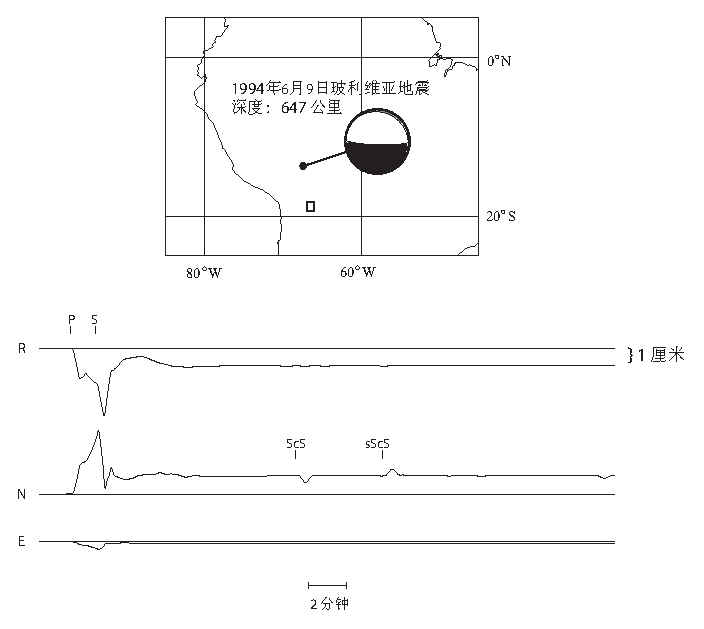
\includegraphics{../figures/chap10/fig19.eps}
\end{center}
\caption[Bolivia near-field]{
\label{fig:10.20}
({\em 上图\/})1994年6月9日玻利维亚深源地震的位置(黑点)和震源机制(沙滩球)。 
({\em 下图\/}) Banjo宽频台阵(上图中方框所示)的台站ST4的近场合成位移地震图。
其中标示了径向(R)、南北(N)和东西(E)分量以及P、S、ScS和~sScS体波讯号。
P波的初动是向下与向北的,而S波的初动是向下与向南的;
断层错动的结果是使该台站向下与向北永久地移动了约一厘米。
P波和S波之间的波形斜坡是形成远震W震相的中场和近场能量的表现,
尤其是在如尼加拉瓜这样的浅源慢地震之后(见图~\ref{fig:10.W-phase})。}
\end{figure}
\index{seismogram|)}%
\index{accelerogram|)}%
图~\ref{fig:10.20}所展示的合成位移记录非常引人注目:
在远场~P~和~S~波之间呈现一个波形斜坡,对应于预期的点震源矩张量响应中中场和近场的贡献~(Aki \& Richards\citeyear{aki&richards80};
Vidale, Goes \& Richards \citeyear{vidale&al95})。
\index{near-field response}%
此外,台站处有一个明显的向下和向北约一厘米的永久位移;
它代表了~(\ref{10.FINAL})~中的因断层上的静态滑移而造成的最终的静态位移~(\ref{10.FINAL})。
\index{static slip}%
\index{slip!static}%
\index{static displacement}%
\index{displacement!static}%
\index{response!static}%
之后到达的远场震相,如南北分量
上的~${\rm ScS}_{\rm SV}$~和~${\rm sScS}_{\rm SV}$,并不影响静态位移~$\bs_{\rm f}(\bx)$。

%\section{Stacking and Stripping}
\section{叠加和剥离}
\index{stacking|(}%
\index{stripping!multiplet|(}%

假定我们现在希望从遍布全球各地的一批地震台站记录到的长周期地震图中分离出一个特定的环
型或球型多态模式。
这可以通过用一种增强目标模式的特征,同时降低噪声的方式合并或{\em 叠加\/}单一大地震的频谱来实现。
在描述这一过程时,我们将忽略非弹性对简正模式本征函数的影响,
同时为简单起见采用~(\ref{10.accfreq})--(\ref{10.Lorentz})~中的频谱近似。
利用矢量球谐函数正交关系~(\ref{8.harm}),
很容易证明实数的矢量振幅~(\ref{10.vectamp})~满足
\eq
\int_\Omega{}{}_n\bA_l(\bx)\cdot{}{}_{n'}\bA_{l'}(\bx)\,d\Omega
=D_{nn'}\delta_{ll'},
\label{eq:10.Ann}
\en
其中积分变量为震中坐标系角度~$\Theta$、$\Phi$,同时
\eqa \label{eq:10.Ann'}
\lefteqn{D_{nn'}=(UU'+VV'+WW')}
\nonumber \\
&&\mbox{}\times[A_0A_0'+\half\sqL^2(A_1A_1'+B_1B_1')
\nonumber  \\
&&\mbox{}\qquad+\half\sqL^2(\sqL^2-2)(A_2A_2'+B_2B_2')].
\ena
为简洁起见,我们在~(\ref{eq:10.Ann'})式右侧省略了辨识模式的下角标~$n$、$n'$ ~和~$l$;不带撇号的量依赖于径向阶数~$n$,带撇号的量则依赖于径向阶数~$n'$。带与不带撇号的本征函数都在接收点半径~$r=a$~处取值。

多态模式~${}_n{\rm S}_l$~或~${}_n{\rm T}_l$~的理想叠加是在地球表面上的加权积分:
\eq
{}_n\Sigma_l(\om)=\int_{\Omega}{}_n\bA_l(\bx)\cdot\ba(\bx,\om)\,d\Omega.
\label{eq:10.stack}
\en
利用~(\ref{eq:10.Ann})~中的结果,我们发现
\eq \label{10.STACK}
\ssSigma(\om)=\ssD\sseta(\om),
\en
其中
\eq
\ssSigma=\left(\begin{array}{c}
\vdots \\
{}_n\Sigma_l \\
\vdots \\
\end{array}\right),\qquad
\sseta=\left(\begin{array}{c}
\vdots \\
{}_n\eta_{\hspace{0.3 mm}l} \\
\vdots \\
\end{array}\right),
\en
\eq
\ssD=\left(\begin{array}{ccc}
       & \vdots  &             \\
\cdots & D_{nn'} & \cdots \\
       & \vdots  &             \\
\end{array}\right).
\en
我们可以将~(\ref{eq:10.stack})~视为一个相位均衡化过程:
首先将复数频谱~$\ba(\bx,\om)$~对齐,然后叠加在一起来增强目标多态模式
~${}_n{\rm S}_l$~或~${}_n{\rm T}_l$~的讯号。
在这一过程中,所有模式类型(球型或环型)以及球谐函数次数~$l$~与目标模式不同的多态模式都被抵消了;只有类型和球谐函数次数相同但径向阶数~$n$~不同的模式被保留下来。

在现实中,没有任何机构会提供资助使我们拥有的三分量地震仪能够对整个地球表面有地毯式的覆盖,因此~(\ref{eq:10.stack})~中的积分永远无法精确计算。
我们必须满足于从位于接收点~$\bx_j,~j=1,2,\ldots,J$~处的全球台网所得到的数目有限的频谱集。
(\ref{eq:10.stack})~中的叠加因而近似为以下求和
\eq \label{10.appstack}
\Sigma(\om)=4\pi J^{-1}\sum_{j=1}^J
\bA(\bx_j)\cdot\ba(\bx_j,\om),
\en
为简单起见我们在此省略了下角标~$n$~和~$l$。
将方程~(\ref{10.appstack})~用下式取代
\eq \label{10.appstack2}
\Sigma(\om)=16\pi^2 I^{-1}J^{-1}
\sum_{i=1}^I\sum_{j=1}^J
\bA_i(\bx_j)\cdot\ba_i(\bx_j,\om),
\en
便可以轻而易举地将来自多个不同地震事件~$i=1,2,\ldots,I$~的数据纳入到叠加中。
$\bA_i(\bx_j)$~是理论的振幅空间变化图像,而~$\ba_i(\bx_j,\om)$~是第~$i$~个震源的观测加速度。
为简单起见,(\ref{10.appstack})--(\ref{10.appstack2})~中我们对所有地震~$\bx_i$~或地震仪~$\bx_j$~分别赋予相同的微分面积元~$d\/\Omega=4\pi I^{-1}$~或~$d\/\Omega=4\pi J^{-1}$;
更普遍地,可能还希望引入一个权重来考虑震源和接收点的不均匀分布。
地理覆盖的不完备性以及其它如分量缺失或噪声过大等实际问题会破坏~(\ref{10.STACK})~中矩阵 ~$\ssD$~理论上的分块对角特性;
因此,在非理想的叠加结果~${}_n\Sigma_l(\om)$~中,
可能存在不同类型或不同球谐函数次数的多态模式,或两者兼有。
在~(\ref{eq:10.Ann})--(\ref{eq:10.Ann'})~中忽略的地球的自转、流体静力学椭率和横向不均匀性也会对这些干扰有所贡献。
尽管有这些困难,叠加仍是一个有用的方法,
因为相较于带来干扰的模式,目标多态模式及其类型和球谐函数次数相同而仅径向阶数不同的模式通常还是得到了增强。

\begin{figure}[!t]
\begin{center}
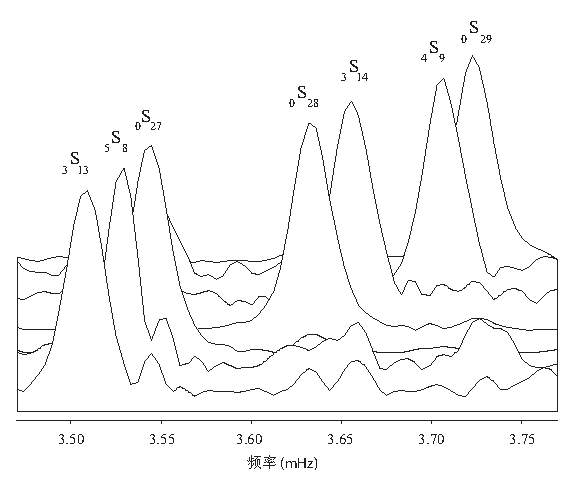
\includegraphics{../figures/chap10/fig20.eps}
\end{center}
\caption[Ruedi 1]{
\label{fig:10.21}
多态模式剥离在~3.50---3.75~毫赫兹窄频段的结果。
目标多态模式{\em 从前向后\/}依次为~${}_3{\rm S}_{13}$、${}_5{\rm S}_{8}$、${}_0{\rm S}_{27}$、
${}_0{\rm S}_{28}$、${}_3{\rm S}_{14}$、${}_4{\rm S}_{9}$
~和~${}_0{\rm S}_{29}$。
每一道曲线中所画的是剥离开来的振幅谱~$|{}_n\eta_{\hspace{0.3 mm}l}(\om)|$。
(由~R. Widmer~提供)。}
\end{figure}

一般而言,固定类型和球谐函数次数~$l$、不同径向阶数的激发较强的模式在频率上有很好的分离,
只有在球型模式中极少数~PKIKP~与~${\rm ScS}_{\rm SV}$~回避相交的频率附近。
因此,在叠加~${}_n\Sigma_l(\om)$~中,要识别~${}_n{\rm S}_l$~和~${}_n{\rm T}_l$~的谱峰几乎没有困难。
一个称作{\em 剥离\/}的附加步骤常常能够进一步改善结果。
由于~$\ssD$~是一已知、对称且正定的矩阵,
因此可以将方程~(\ref{10.STACK})~反演来恢复单个的共振谱峰:
\eq
\sseta(\om)=\ssD^{-1}\ssSigma(\om).
\label{eq:10.resonance}
\en
在~(\ref{eq:10.resonance})式的实际应用中,
为抑制数值不稳定,
通常用对~$\ssD$~做奇异值分解所得到的广义逆~$\ssD^{-\mbox{\scriptsize g}}$~来取代 ~$\ssD^{-1}$。
\index{generalized inverse}%
由此得到的列矢量~$\sseta(\om)$~的每一个分量~${}_n\eta_{\hspace{0.3 mm}l}(\om)$~被称为一个{\em multiplet 多态模式剥离条带\/}。
\index{multiplet strip}%
\index{stripping!multiplet}%
通过将每个剥离条带用~(\ref{10.Lorentz})~中的洛伦兹谱峰做最小二乘拟合,可以测量简并的本征频率~${}_n\om_l^{\rm S}$和~${}_n\om_l^{\rm T}$。
一系列微小的细节都必须仔细地关注到,才能够成功地实施叠加和剥离,并使偏差最小化~(Widmer \citeyear{widmer91})。
这两种方法都需要知道每个震源的位置~$\bx_{\rm s}$~和矩张量~$\bM$。

Mendiguren (\citeyear{mendiguren73})~是第一个将此叠加原理应用于全球地震台网的地震学家。
他使用了~${\rm sgn}\,\bA(\bx_j)$~而不是~$\bA(\bx_j)$~作为~(\ref{10.appstack})~中的权重,
也就是说,他在求和之前直接将激发振幅为负的记录做极性反转。
这一开创性的研究中所使用的地震图是人工数字化的世界标准地震台网~(WWSSN)~的1970年7月31日哥伦比亚深源地震的记录。
\index{Colombia 1970 earthquake}%
之后由\textcite{gilbert&dziewonski75}发展了前述的叠加和剥离程序;
他们测量了~800~多个地球自由振荡的简并本征频率,
并共同利用已有数据构建了两个与观测相符的~SNREI~地球模型---1066A~和~1066B。
随后,又通过拟合基本上相同的约~1000~个简正模式的本征频率,加上另外~500~个汇总的走时测量值以及~100~个多态模式的品质因子数据,得到了横向各向同性且非弹性的~PREM~模型~(Dziewonski \& Anderson \citeyear{dziewonski&anderson81})。

\begin{figure}[!t]
\begin{center}
\scalebox{0.8}{
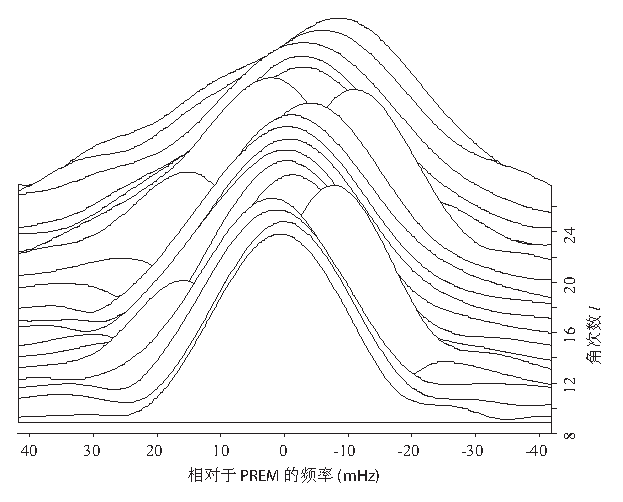
\includegraphics{../figures/chap10/fig22.eps}
}
\end{center}
\caption[Ruedi 3]{
\label{fig:10.23}
基阶球型模式~${}_0{\rm S}_{8}$ ({\em 前\/})~至~${}_0{\rm S}_{30}$ ({\em 后\/}) 的剥离条带~$|{}_n\eta_{\hspace{0.3 mm}l}(\om-\om_{\rm PREM})|$。 请注意,横坐标的频率是反转的,因而左边~$\om>\om_{\rm PREM}$,右边~$\om<\om_{\rm PREM}$ 。(由R. Widmer提供)。}
\end{figure}
\begin{figure}[!b]
\begin{center}
\scalebox{0.8}{
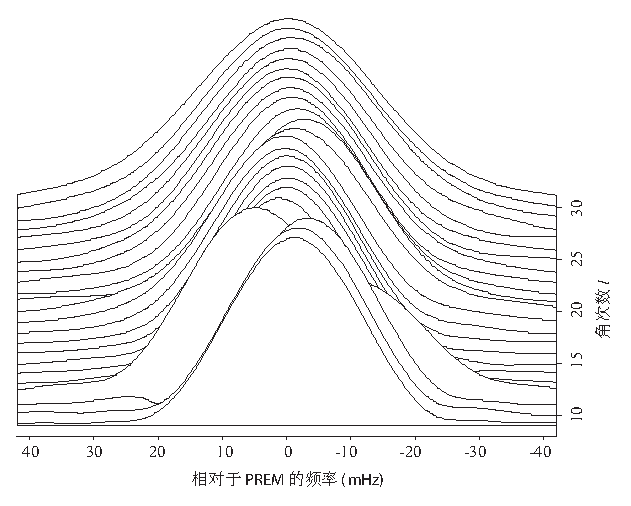
\includegraphics{../figures/chap10/fig21.eps}
}
\end{center}
\caption[Ruedi 2]{
\label{fig:10.22}
基阶环型模式~${}_0{\rm T}_{8}$~({\em 前\/})~至~${}_0{\rm T}_{26}$~({\em 后\/})~的剥离条带 ~$|{}_n\eta_{\hspace{0.3 mm}l}(\om-\om_{\rm PREM})|$。(由R. Widmer提供)。}
\end{figure}

近期的工作聚焦在对偶尔发生的模式识别错误进行校正,
更重要的是通过分析更多的数字地震记录来减小本征频率的测量误差。
图~\ref{fig:10.21}很好地展示了高质量的现代数字剥离条带。
在~3.50--3.75~毫赫兹这一狭窄频带中,
径向高阶模式~${}_3{\rm S}_{13}$、${}_5{\rm S}_{8}$、
${}_3{\rm S}_{14}$~和~${}_4{\rm S}_9$~与激发更强的基阶模式~${}_0{\rm S}_{27}$, ${}_0{\rm S}_{28}$~和~${}_0{\rm S}_{29}$~被异常完美地分离开来。
图~\ref{fig:10.22}和~\ref{fig:10.23}显示在~$1.5\hspace{0.2 mm}$--$\hspace{0.2 mm}4.0$ ~毫赫兹频带内的所有基阶球型和环型模式都可以被成功地剥离;
图中每个谱峰都是用相对于各自在~PREM~中的频率移动了的频率刻度~$\om-\om_{\rm PREM}$~所画的。
这些观测频率残差曲线之间独特的偏移是地球自转的表现;
由于球型与环型多态模式之间的科里奥利耦合,造成了频率相近且球谐函数次数相邻的两个模式~(如~${}_0{\rm S}_{11}\hspace{0.2 mm}$--$\hspace{0.2 mm}
{}_0{\rm T}_{12}$~和~${}_0{\rm S}_{19}\hspace{0.2 mm}$--$\hspace{0.2 mm}
{}_0{\rm T}_{20}$)~的剥离条带之间“相斥”。
\index{repulsion}%
在第~14.3.2~节中,我们会看到对这种效应在理论上已经有很清楚的理解,因此而造成的偏差是可以消除的。Masters \& Widmer(\citeyear{masters&widmer95})~汇集了包扩~600~多个经过科里奥利效应校正后的本征频率一组现代的高质量数据。图~\ref{fig:10.25}显示了这些测量到的模式。
其中大多数测量都是用从数千道记录得到的多态模式剥离条带做的。
\index{stacking|)}%
\index{stripping!multiplet|)}%

\begin{figure}[!b]
\begin{center}
\scalebox{0.85}
{
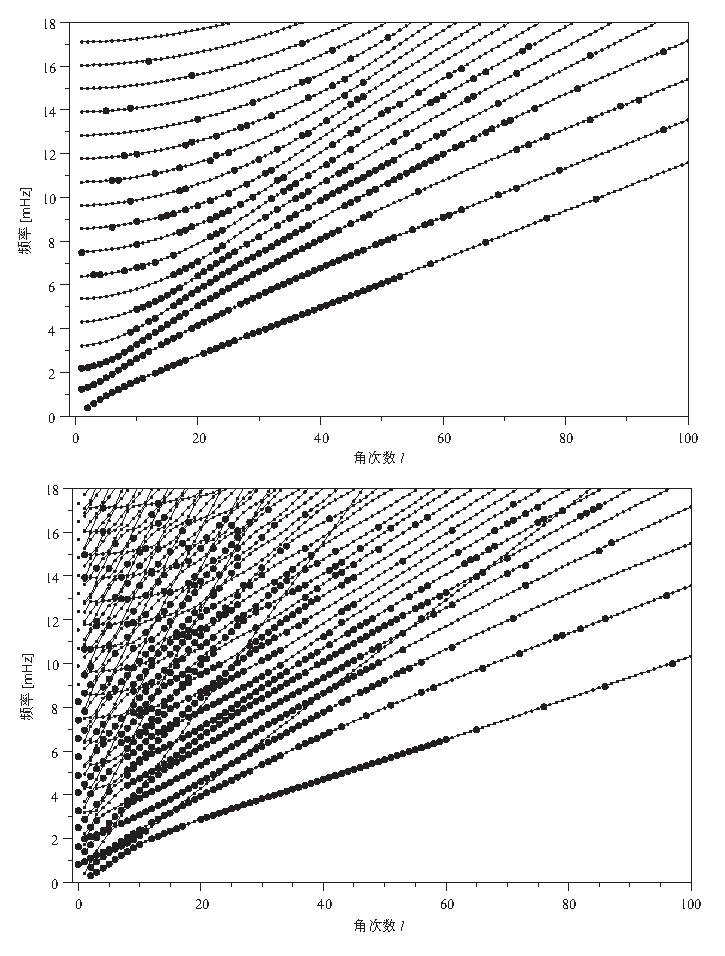
\includegraphics{../figures/chap10/fig23.eps}
}
\end{center}
\caption[Guy modes]{
\label{fig:10.25}
环型模式({\em 上图\/})和球型模式 ({\em 下图\/}) 频散图中的大圆点标示其简并本征频率目前认为是"已被可靠地确定"。
对图中的许多高精度数据,PREM并未给予足够好的拟合。(由R. Widmer提供)。}
\end{figure}

\renewcommand{\thesection}{$\!\!\!\raise1.3ex\hbox{$\star$}\!\!$
\arabic{chapter}.\arabic{section}}
%\section{Alternatives to Mode Summation}
\section{模式叠加的替代方法}
\renewcommand{\thesection}{\arabic{chapter}.\arabic{section}}

在本节中,我们将简要介绍用简正模式叠加计算球对称地球合成地震图的两种替代方法。
这两种方法都是在频域中直接求解对矩张量源的响应,
并通过傅里叶反变换的数值计算,得到时间域的位移~$\bs(\bx,t)$~或加速度~$\ba(\bx,t)$。
这种直接方法的优点是频率采样间隔可根据眼前的应用进行调整;
计算量与频率采样数目成正比,从而与需要合成的地震图的长度成正比。
它可以用于某些高频应用中,当需要的地震图在时间上较短,如单一体波讯号。
而在简正模式方法中,相邻本征频率间的间隔显然是不可改变的;
最费气力的一步是最初要构建一个完备的本征频率、多态模式品质因子和本征函数的目录。
有了这样的目录,用模式叠加计算短时段地震图比长時段少用不了多少时间。

第一个直接方法的出发点是非齐次动量方程
\eqa \label{10.DSM1}
\lefteqn{-\om^{2\!}\rho\hspace{0.2 mm}\bs-\bdel\cdot\bT
+(4\pi G\rho^2s_r)\brh+\rho\bdel_{\!}\phi} \nonumber \\
&&\mbox{}+\rho g[\bdel_{\!}s_r-(\bdel\cdot\bs+2r^{-1}s_r)\brh] \nonumber \\
&&\mbox{}\qquad=-[\pi\delta(\om)+(i\om)^{-1}]\,
\bM\!:\!\bdel\delta(\bx-\bx_{\rm s}).
\ena
方程~(\ref{10.DSM1})~左侧包含了相应的齐次方程~(\ref{eq:8.smeq})~左边的所有项。右边则是与地震相对应的等效力~$\bef(\bx,\om)$。
$\pi\delta(\om)+(i\om)^{-1}$~是~Heaviside~函数~$H(t)$~的傅里叶变换;
如有必要,可以用依赖于频率的矩张量~$\bM(\om)$~来考虑更普遍的震源时间函数。
将位移~$\bs(\bx,\om)$~和力~$\bef(\bx,\om)$~用矢量球谐函数~$\bP_{lm}$、$\bB_{lm}$~和 ~$\bC_{lm}$~展开,
我们可以得到与环型、球型和径向模式所满足的方程~(\ref{eq:8.U})--(\ref{eq:8.W})~类似的 的三个二阶常微分方程,
把相应的齐次一阶方程组~(\ref{eq:8.tor1})--(\ref{eq:8.tor2}),
(\ref{eq:8.foU})--(\ref{eq:8.foK}),~(\ref{eq:8.Ufl})--(\ref{eq:8.Kfl})
~和~(\ref{eq:8.Urad})--(\ref{eq:8.Rrad}) 简写为~$\dot{\ssy}=\ssA\ssy$,
我们需要求解一系列以下形式的非齐次系统
\eq \label{10.DSM2}
\dot{\ssy}=\ssA\ssy+\ssz_1\delta(r-r_{\rm s})+
\ssz_2\dot{\delta}(r-r_{\rm s}),
\en
其中矢量~$\ssz_1(\om)$~和~$\ssz_2(\om)$~依赖于震源机制~$\bM$~和地理位置~$\theta_{\rm s},\phi_{\rm s}$。非齐次项的存在破坏了~$\ssy(r,\om)$~的~$2l+1$~重简并;
将震源置于极点 ($\theta_{\rm s}\rightarrow 0$) 会大大减小计算上的负担,
因为$\ssz_1(\om)$和$\ssz_2(\om)$只有在级数 $m=0$、$m=\pm 1$ 和 $m=\pm 2$时不为零。
方程~(\ref{10.DSM2})的解的形式为$\ssy(r,\om)=\ssv(r,\om)
+\ssz_2(\om)\delta(r-r_{\rm s})$, 
其中$\dot{\ssv}=\ssA\ssv+
(\ssz_1+\ssA\ssz_2)\delta(r-r_{\rm s})$。
矢量 $\ssv(r,\om)$ 可以借由数值积分获得;
非齐次项导致在震源深度~$r=r_{\rm s}$~处有一个不连续跃变~$\ssz_1(\om)+\ssA(r_{\rm s},\om)\ssz_2(\om)$。
在自由表面~$r=a$~和任何固-液不连续面~$r=d_{\rm FS}$~上的边界条件仍然是与环型、球型和径向本征模式所满足的完全相同的~(\ref{eq:8.btor2})、~(\ref{eq:8.bfoa})--(\ref{8.Fried})~和~(\ref{8.radbc})。
(\ref{10.DSM2})~中系统的刚性带来的数值不稳定性 可以像在齐次情形中一样,通过求解结果矩阵的余子式而不是矩阵本身来克服。
非弹性可以通过在系数矩阵 ~$\ssA(r,\om)$~中使用复数且依赖频率的弹性参数~$\kappa_0[1+iQ_{\kappa}^{-1}
+\twoinvpi Q_{\kappa}^{-1}\ln
(\om\hspace{-0.2 mm}/\hspace{-0.2 mm}\om_0)]$和
$\mu_0[1+iQ_{\mu}^{-1}
+\twoinvpi Q_{\mu}^{-1}\ln
(\om\hspace{-0.2 mm}/\hspace{-0.2 mm}\om_0)]$来考虑。
Friederich \& Dalkolmo
(\citeyear{friederich&dalkolmo95})~对这一{\em 直接径向积分\/}方法在数值上的实现做了介绍。
\index{direct radial integration}%
他们讨论了使频率混叠假象最小化的策略,并展示了与模式叠加地震图的比较,以确立他们结果的正确性。

第二种替代方法是基于第~\ref{7.sec.need13}节中所简要讨论的{\em 直接代数\/}方法。
\index{direct solution method!SNREI Earth}%
通过选择与矢量球谐函数~$\bP_{lm}$、$\bB_{lm}$~和~$\bC_{lm}$~成比例的基函数,
将动能和势能矩阵~$\ssT$~和~$\ssV(\om)$~分解为给定球谐次数~$l$~的
环型、球型或径向独立矩阵。
例如,环型矩阵的分量为
\eq \label{10.DSM3}
T_{kk'}=\int_b^s\rho X_kX_{k'}\,r^2dr,
\en
\eqa \label{10.DSM4} \lefteqn{
V_{kk'}(\om)=\int_b^s\mu_0[1+iQ_{\mu}^{-1}
+\twoinvpi Q_{\mu}^{-1}\ln
(\om\hspace{-0.2 mm}/\hspace{-0.2 mm}\om_0)]} \nonumber \\
&&\mbox{}\times[(r\dot{X}_k-X_k)
(r\dot{X}_{k'}-X_{k'})
+(l-1)(l+2)X_kX_{k'}]\,dr,
\ena
其中~$X_k(r)$~为我们尚未指定的径向基函数。
局部三角形或线性样条是普遍的选择,因
为它们形式简单且导致稀疏矩阵:
\eq \label{10.Gsplines}
X_k(r)=\left\{\begin{array}{ll}
(r-r_{k-1})/(r_k-r_{k-1}) & \mbox{如果 $r_{k-1}\leq r\leq r_k$} \\
\vspace{-1.0 mm} & \vspace{-1.0 mm} \\
(r_{k+1}-r)/(r_{k+1}-r_k) & \mbox{如果 $r_k\leq r\leq r_{k+1}$} \\
\vspace{-1.0 mm} & \vspace{-1.0 mm} \\
0 & \mbox{其它情况,} \end{array} \right
\en
其中~$b=r_1<r_2<\cdots<r_K=s$。
(\ref{10.Gsplines})~式中的第一行和第二行分别在端点~$k=1$~和~$k=K$~处不必考虑。
将震源置于极点~($\theta_{\rm s}\rightarrow 0$)~处仍然是有利的,
因为它将源点矢量~$\sss$~局限为级数~$|m|\leq 2$~的分量。
将~(\ref{B.Psipsi})~中的变换用于~($\theta_{\rm s}\rightarrow 0$)~的极限关系式~(\ref{D.eps7})--(\ref{D.eps12}),我们得到环型矩阵的非零分量:
\eq
s_{k\,\pm 1}=\left\{\begin{array}{l}
-\left(\frac{2l+1}{8\pi}\right)^{1/2}
M_{r\theta}(\dot{X}_k-r^{-1}X_k)_{r=r_{\rm s}} \\
\vspace{-1.0 mm} \\
\hspace{3.4 mm}\left(\frac{2l+1}{8\pi}\right)^{1/2}
M_{r\phi}(\dot{X}_k-r^{-1}X_k)_{r=r_{\rm s}},  \end{array} \right.
\en
\begin{displaymath}
s_{k\,\pm 2}=\left\{\begin{array}{l}
\hspace{0.3 mm}\half\left(\frac{2l+1}{8\pi}\right)^{1/2}\sqrt{(l-1)(l+2)}
\,(M_{\theta\theta}-M_{\phi\phi})(r^{-1}X_k)_{r=r_{\rm s}} \\
\vspace{-1.0 mm} \\
-\left(\frac{2l+1}{8\pi}\right)^{1/2}\sqrt{(l-1)(l+2)}\,
M_{\theta\phi}(r^{-1}X_k)_{r=r_{\rm s}}. \end{array} \right.
\end{displaymath}
相应的环型的接收点矢量~$\ssr$~分量为
\eq
r_{k\,\pm 1}=X_k(r)\,\bnuh\cdot\bC_{l\,\pm 1}(\theta,\phi),
\en
\eq
r_{k\,\pm 2}=X_k(r)\,\bnuh\cdot\bC_{l\,\pm 2}(\theta,\phi).
\en
要得到次数为~$l$、级数为~$m=\pm 1,\pm 2$~的响应,
我们求解依赖频率的线性方程
\eq \label{10.DSM7}
[\ssV(\om)-\om^2\ssT]\ssd(\om)=\sss.
\en
因而加速度~$a(\om)=\bnuh\cdot\ba(\bx,\om)$~可以用环型响应矢量~$\ssd(\om)$~表示为
\eq \label{10.DSM8}
a(\om)=i\om\ssr^{\rm T}\ssd(\om).
\en
Cummins, Geller, Hatori \& Takeuchi
(1994)~展示了用方程~(\ref{10.DSM3})--(\ref{10.DSM8})~的完全弹性、复数球谐函数形式得到的
数值结果。
他们介绍了一些小的修改,能够在给定的结点间隔下提高计算精度。
对相应的球型公式推导,
由于要考虑固态的内核和地幔~$\earth_{\rm S}$~与
液态的外核和海洋~$\earth_{\rm F}$~中自由度数目的不同,
以及固-液边界~$d_{\rm FS}$~上可能的滑动,因而会更加复杂~(Cummins, Geller \& Takeuchi 1994;
Takeuchi, Geller \& Cummins \citeyear{takeuchi&al96})
\nocite{cummins&al94a} \nocite{cummins&al94b}。
Cummins (\citeyear{cummins97})~证明了球对称地球直接求解法程序的正确性;
在他复制的图~\ref{fig:10.20}的径向近场地震图中,波形一一完美重叠,令人印象深刻。